% !Mode:: "TeX:UTF-8"
%%% Local Variables:
%%% mode: latex
%%% TeX-master: t
%%% End:

\documentclass[type=master]{thuthesis}
% 选项:
%   type=[bachelor|master|doctor|postdoctor], % 必选
%   secret,                                   % 可选
%   pifootnote,                               % 可选(建议打开)
%   openany|openright,                        % 可选,基本不用
%   arial,                                    % 可选,基本不用
%   arialtoc,                                 % 可选,基本不用
%   arialtitle                                % 可选,基本不用

% 所有其它可能用到的包都统一放到这里了,可以根据自己的实际添加或者删除。
\usepackage{thuthesis}
\usepackage{bm}
\usepackage{algorithm}
\usepackage{algpseudocode}
\usepackage{makecell}

\usepackage{tikz}
\usetikzlibrary{arrows,shapes,positioning}

% 算法相关
\floatname{algorithm}{算法}
\makeatletter
\@addtoreset{algorithm}{chapter}% algorithm counter resets every chapter
\makeatother
\renewcommand{\thealgorithm}{\thechapter.\arabic{algorithm}}% Algorithm # is <chapter>.<algorithm>
\algnewcommand\algorithmicinput{\textbf{输入:}}
\algnewcommand\INPUT{\item[\algorithmicinput]}
\algnewcommand\algorithmicoutput{\textbf{输出:}}
\algnewcommand\OUTPUT{\item[\algorithmicoutput]}
\algnewcommand\algorithmicinit{\textbf{初始化:}}
\algnewcommand\INIT{\item[\algorithmicinit]}

%表格相关
\newcolumntype{Y}{>{\centering\arraybackslash}X}
\newcolumntype{I}{!{\vrule width 1.5pt}}

% 定义所有的图片文件在 figures 子目录下
\graphicspath{{figures/}}

% 可以在这里修改配置文件中的定义。导言区可以使用中文。
% \def\myname{薛瑞尼}
\begin{document}

%%% 封面部分
\frontmatter
\thusetup{
  %******************************
  % 注意:
  %   1. 配置里面不要出现空行
  %   2. 不需要的配置信息可以删除
  %******************************
  %
  %=====
  % 秘级
  %=====
  secretlevel={绝密},
  secretyear={2100},
  %
  %=========
  % 中文信息
  %=========
  ctitle={短波语音信号的质量评价算法及自动选路系统研究},
  cdegree={工学硕士},
  cdepartment={电子工程系},
  cmajor={信息与通信工程},
  cauthor={陈晔},
  csupervisor={谷源涛副教授},
  %cassosupervisor={陈文光教授}, % 副指导老师
  %ccosupervisor={某某某教授}, % 联合指导老师
  % 日期自动使用当前时间,若需指定按如下方式修改:
  cdate={二〇一七年六月},
  %
  % 博士后专有部分
  %cfirstdiscipline={计算机科学与技术},
  %cseconddiscipline={系统结构},
  %postdoctordate={2009年7月——2011年7月},
  %id={编号}, % 可以留空: id={},
  %udc={UDC}, % 可以留空
  %catalognumber={分类号}, % 可以留空
  %
  %=========
  % 英文信息
  %=========
  etitle={Study on Preprocessing Technique and Background Model in Drosophila Recognition and Behavior Analysis},
  % 这块比较复杂,需要分情况讨论:
  % 1. 学术型硕士
  %    edegree:必须为Master of Arts或Master of Science(注意大小写)
  %             “哲学、文学、历史学、法学、教育学、艺术学门类,公共管理学科
  %              填写Master of Arts,其它填写Master of Science”
  %    emajor:“获得一级学科授权的学科填写一级学科名称,其它填写二级学科名称”
  % 2. 专业型硕士
  %    edegree:“填写专业学位英文名称全称”
  %    emajor:“工程硕士填写工程领域,其它专业学位不填写此项”
  % 3. 学术型博士
  %    edegree:Doctor of Philosophy(注意大小写)
  %    emajor:“获得一级学科授权的学科填写一级学科名称,其它填写二级学科名称”
  % 4. 专业型博士
  %    edegree:“填写专业学位英文名称全称”
  %    emajor:不填写此项
  edegree={Master of Science},
  emajor={Information and Communication Engineering},
  eauthor={Hou Qi},
  esupervisor={Associate Professor Gu Yuantao},
  %eassosupervisor={Chen Wenguang},
  % 日期自动生成,若需指定按如下方式修改:
  edate={April, 2016},
  %
  % 关键词用“英文逗号”分割
  ckeywords={果蝇, 背景模型, 行为分析},
  ekeywords={Drosophila, Background Model, Behavior Analysis}
}

% 定义中英文摘要和关键字
\begin{cabstract}
  动物行为学研究是生物学研究的一个重要领域,动物行为学通过观察、计数研究动物的行为。果蝇的基因结构简单、身体结构简单,成为动物行为学研究中的重点研究对向。果蝇行为学研究需要分析大量的果蝇视频数据,手工标定需要花费大量的人力成本,且手工标定可能存在标准不一致等问题,用计算机自动分析果蝇的行为成为一个可行解决方案。目前已经存在自动分析果蝇行为的研究。果蝇行为识别的主要流程包括果蝇活动台提取、果蝇身体轮廓提、果蝇特征提取、行为模式识别等步骤。目前的研究一般受限于特定的实验条件和拍摄环境,往往难以适应其他实验环境。其中,果蝇轮廓提取步骤往往是其中的制约因素。此外,果蝇活动台提取步骤也限制了整个流程自动化的程度。为此,本文提出一种特定排列模式下的果蝇活动台提取算法和一种基于背景模型的轮廓提取算法。主要工作可以概括为以下几个方面:

  首先,本文提出一种特定排列模式下的果蝇活动台轮廓提取算法。通过圆检测等形状检测方式提取活动台的位置和大小,进而根据果蝇活动台的排列方式,对果蝇活动台的位置进行进一步的调整。

  其次,本文提出一种基于背景模型的果蝇轮廓提取算法,可以从视频中提取果蝇的身体和翅膀。算法采用单高斯模型作为背景模型,通过亮度畸变区分果蝇翅膀和身体。初步建模后分离果蝇身体和活动台背景;然后在对活动台单独进建模的基础上,得到最终的背景模型。

  然后,在背景模型的基础上,进行果蝇打架行为分析,验证了本文提出的算法的有效性。

  最后,搭建果蝇行为识别网站,并介绍果蝇行为识别软件的程序部分和网站部分,以及网站的基本使用说明。

  本文提出的基于特定排列模式的果蝇活动台算法提高了果蝇自动分析的自动化程度;基于背景模型的果蝇轮廓提取算法具有较好的鲁棒性,可以适用于不同拍摄环境,有助于提高自动化果蝇行为分析的适用范围。此外,该模型还可以应用于动物行为学中对其他动物的研究。


\end{cabstract}

% 如果习惯关键字跟在摘要文字后面,可以用直接命令来设置,如下:
% \ckeywords{\TeX, \LaTeX, CJK, 模板, 论文}

\begin{eabstract}

In biology research, ethology is an important area. By observing the behavior of animals, ethologists get the internal mechanism of animals. Drosophila has a simple genetic structure as well as a simple body structure, which makes it an important role in ethology. In traditional research, much manpower is needed to watch the videos and count the behaviors. Also, there may be different standards for behavior detection, which makes it hard to generalize. With the development of computer vision and machine learning, analyzing the fly video by computer becomes possible.

The main procedure includes drosophila chamber extraction, drosophila body contour extraction, drosophila feature extraction, and drosophila behavior pattern recognition. But the current study is generally limited by specific environments, and cannot generalize to other laboratory circumstance. Drosophila contour extraction step is often the restrictive factors, followed by drosophila chamber extraction step. To solve this problem, we propose a method to extract drosophila chambers based on the specific layout pattern. For the contour extraction step, we propose a drosophila contour extraction algorithm based on background model. The main work can be summarized as follows:

Firstly, this paper presents a drosophila chamber extraction algorithm based on specific layout pattern. First extract the chambers by shape detection method such as hough circle detection, then cluster the shapes to get the position of chambers, then adjust the position according to the layout of the chambers with transformation of coordinates.

Secondly, this paper presents a drosophila contour extraction algorithm based on background model, which extracts the body and wings of drosophila from the video. The algorithm uses a single Gaussian distribution as the background model, and distinguishes the drosophila wings and body by luminance distortion. After the preliminary background modeling, we can separate the drosophila body from the containers. Then we do background modeling on the container only, which makes a better background model for drosophila contour extraction.

Then, we analyze the fly fighting behaviors based on the algorithm, and it turns out to be effective.

Finally, we build a website that provide fly behavior analysis service, also we make a detailed introduction to the DetectFly software and the website, as well as the basic instructions for the website.

In conclusion, the drosophila chamber extraction algorithm reduce the manual operation in drosophila analysis. The contour extraction algorithm proves to be robust in different videos from different cameras, which helps to improve the application scope of  automated drosophila behavior analysis. In addition, the model can be applied to animal studies in other animals.

\end{eabstract}

% \ekeywords{\TeX, \LaTeX, CJK, template, thesis}

% 如果使用授权说明扫描页,将可选参数中指定为扫描得到的 PDF 文件名,例如:
% \makecover[scan-auth.pdf]
\makecover

%% 目录
\tableofcontents

%% 符号对照表
% !Mode:: "TeX:UTF-8"
%%% Local Variables:
%%% mode: latex
%%% TeX-master: t
%%% End:

\begin{denotation}[3cm]
\item[$I$]  视频中的图像帧
\item[$param_1$]  Hough圆检测的Canny算子阈值参数
\item[$param_2$]  Hough圆检测的累加器阈值参数
\item[$A$]  图像坐标系向理想坐标系的变换矩阵
\item[$B$]  理想坐标系向图像坐标系的变换矩阵
\item[$\textrm{M}_1$] 简单单高斯背景模型
\item[$\textrm{M}_2$] 果蝇活动台的精确背景模型
\item[$\mu$]    背景模型$\textrm{M}_1$中视频帧的均值
\item[$\sigma^2$]   背景模型$\textrm{M}_1$中视频帧的方差
\item[$\alpha$] $\textrm{M}_1$中视频帧的亮度畸变
\item[$\textrm{RMS}(\alpha)$] $\textrm{M}_1$中视频亮度畸变的均方差
\item[$\mu'$]   背景模型$\textrm{M}_2$中活动台的均值
\item[$\sigma^{\prime 2}$] 背景模型$\textrm{M}_2$中活动台的方差
\item[$\alpha'$] $\textrm{M}_2$中视频帧的亮度畸变
\item[$\textrm{RMS}(\alpha')$] $\textrm{M}_2$中视频亮度畸变的均方差
\item[$I_{body}$]    果蝇身体的二值图像
\item[$I_{wing}$]    果蝇翅膀的二值图像
\item[$\tau_{body}$] 提取果蝇身体的阈值
\item[$\tau_{wing}$] 提取果蝇翅膀的阈值
\item[$a$]    视频中的果蝇身体长度的一半
\item[$b$]    视频中的果蝇身体宽度的一半
\item[$\vec{\bm p}$]    果蝇特征点坐标
\end{denotation}



%%% 正文部分
\mainmatter

\tikzstyle{block} = [rectangle, draw, text width=15em,  text centered, rounded corners, minimum height=3.5em]
\tikzstyle{arrow} = [thick, draw, -latex']

%引言
% !Mode:: "TeX:UTF-8"
%%% Local Variables:
%%% mode: latex
%%% TeX-master: t
%%% End:

\chapter{引言}
\label{chapter:introduction}

\section{研究背景}

短波通信又称高频通信,是指使用频率范围在高频(HF)的无线电进行通信的方式\cite{董彬虹2007短波通信的现状及发展趋势}。短波通信主要利用天波电离层反射,所以无需中继站即可实现远距离通信,具有机动性强、设备成本低、对基础设施依赖小的优点,因此被广泛应用于广播、军事和抢险救灾等领域。

而同时,短波通信的缺陷也非常突出,因为受电离层变化和多径传播等因素的影响,短波通信的信道非常不稳定,导致其通信质量起伏较大,影响通信的稳定性。应对这一问题,军事中应用短波语音进行地空通信时,目前有一种解决方案:如图~\ref{fig:sys_struct}所示,在地面不同地点建立多个短波信号接收基站,接收来自空中飞机的短波语音。再将这多路信号汇总到一起,由人工选择一路质量最优的信号接入给地面指挥人员。人工选择需要的人工成本高,且稳定性和可靠性都不高,亟待使用算法代替人工。本文旨在通过对一系列算法及系统的研究,使用算法替代该方案中的人工选择步骤。

\begin{figure}
\centering
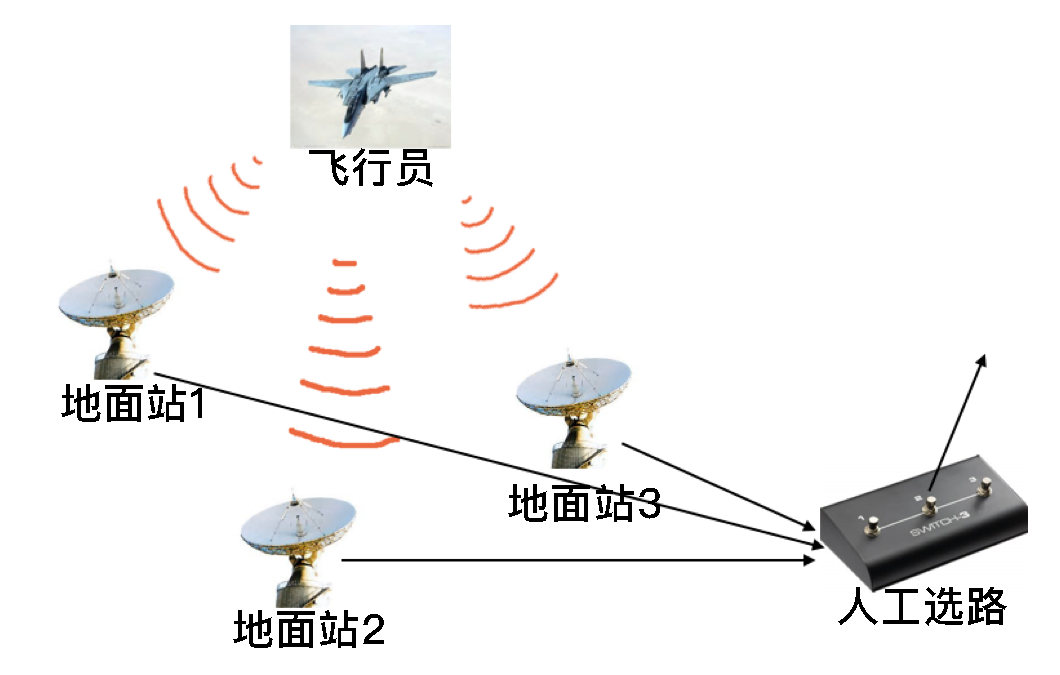
\includegraphics[width=0.8\textwidth]{sys_struct}
\caption{军事应用中的一种地空短波通信系统\label{fig:sys_struct}}
\end{figure}

\section{研究现状}


\subsection{背景模型及其在果蝇身体检测中的应用}


\section{研究目标和研究内容}

本文的主要目标在于研究果蝇活动台分割算法和果蝇轮廓提取算法,提升算法的鲁棒性,提升果蝇行为识别算法的应用范围。本文的研究内容主要包括:
\begin{enumerate}
\item 针对现有果蝇活动台提取算法的精确度较低的问题,本文引入了果蝇活动台的排列模式,通过将图像中的活动台和理想排列模式之间建立一一映射,去除果蝇活动台提取过程中的噪声。此外,对于不按照固定模式排列的果蝇活动台,引入自适应机制,减少该步骤中的人工干预;
\item 果蝇行为视频的实验环境和拍摄条件差异给果蝇轮廓提取带来很大的困难,针对此问题,本文提出一种果蝇轮廓提取算法,采用单高斯模型作为背景模型,通过亮度畸变区分果蝇翅膀和身体。初步建模后分离果蝇身体和活动台背景;然后在对活动台单独进建模的基础上,得到精确的背景模型用于轮廓提取。
\item 创建果蝇行为识别网站,对果蝇研究单位提供果蝇视频分析服务。
\end{enumerate}

\section{论文结构和内容概述}

本文剩余部分的结构如下所示:

第2章主要介绍短波语音客观质量评价算法。介绍了两种客观评价算法,一种是基于语谱图噪音模型的算法,另一种是基于人工神经网络自编码器的算法。前者根据短波语音的噪音特征设计,对于短波语音的质量评价效果非常好,但是算法针对性太强,迁移到其他领域的语音信号时,需要重新分析对应的噪音特征;而后者通过自编码器学习纯净语音信号的语谱特征,可以方便地迁移到其他领域。

第3章主要介绍多路短波语音自动选路系统。首先介绍了多路语音时间对齐算法,然后介绍了基于此算法以及第2章介绍的客观评价算法的自动选路系统。

第4张介绍了语音质量在线主观评价辅助系统,首先介绍了系统的功能和使用方法,然后介绍了系统开发和部署环境及运行原理。

第5章介绍了实验的情况。通过两组实验分别验证了第2章所提算法及第3章所提系统的实际效果,在短波语音数据集上对比了本文所提算法与两种标准质量评价算法的表现。

第6章对本文工作进行总结,并对将来可能的研究方向进行展望。




\chapter{短波语音客观质量评价算法}
\label{chap:algorithms}

为了能够从多路短波语音中自动切换选择,需要使用算法对各路短波语音的质量进行评价。由于系统没有原始语音作为参考,所以需要的客观质量评价算法是单端的客观评价算法。现有的语音客观质量评价算法主要针对VoIP应用、语音编解码系统、语音降噪系统等场景,这些场景中的语音质量相较短波语音要好,信噪比较高。直接将现有的算法应用到短波语音上难以取得良好的评价结果。所以本章提出了两种可用在短波语音上的客观质量评价算法

\section{基于语谱图噪音模型的客观质量评价算法}

\subsection{启发性思路} \label{section:alg1-1}

语谱图是一种从频域对语音信号进行分析的工具,将语音信号转换到频域进行分析,需要使用短时傅里叶变换(STFT)。给定一个时间宽度很短的窗函数,语音信号的STFT定义为\ref{eq:stft}

\begin{equation}\label{eq:stft}
F_{STFT}(t, f) = \int_{-\infty}^{+\infty}x(u)g^*(u-t)e^{-j2\pi fu}du
\end{equation}

由于窗函数在时域有限,使得短时傅里叶变换具有局部特性,能够反映指定时刻的局部频谱信息。
实际应用中,需要使用离散化的短时傅里叶变换,取$t=mT, f=nF$,其中$T$和$F$分别为时间和频率的采样间隔,$m,n=0,1,2,...,M-1$,$M$是采样点数。则离散形式的STFT为\ref{eq:dstft}

\begin{equation}\label{eq:dstft}
F_{STFT}(m, n) = \sum_{k=0}^{N-1}x(kT)g^*((k-m)T)e^{-j2\pi nk/N}
\end{equation}

$F_{STFT}(m, n)$反映的是$mT$时刻,$nF$频率附近的局部频谱信息。

根据对于人耳听觉特性的一些研究,人耳对于声音信号的相位特性并不敏感,但是对于幅度特性敏感,并且人耳对于声音响度的感受是与信号能量的对数成正比的。所以对离散短时傅里叶变换得到的结果,只保留幅值能量,并进一步做取对数的处理,得到的二维信息可以用图像展示,称之为语谱图,定义为\ref{eq:log_dstft}

\begin{equation}\label{eq:log_dstft}
G(m, n) = log(|F_{STFT}(m, n)|^2)
\end{equation}

语谱图反映了语音信号在不同时间、不同频率上的能量大小,承载了语音所包含的信息。高质量语音的语谱图上有着清晰的结构特征,包括基音部分的能带,各种高次谐波的能带;而带有噪音的语谱图则没有模糊不清。在短波语音信号上亦是如此。如图~\ref{fig:timefreq}所示,从左到右是质量由低到高五组短波语音的语谱图,分别对应主观评分1-5分。从语谱图上可以看到条带状的语音部分越来越突出和明显。图~\ref{fig:timefreq-thr0.3}是由图~\ref{fig:timefreq}中各个语谱图以0.3为阈值转化为二值图像的结果,图中可以更加明显的看出质量越好的语音信号,条带状的纯净语音部分越清楚,而质量较差的语音信号,则因为存在噪音连成模糊的一片。

\begin{figure}
\centering
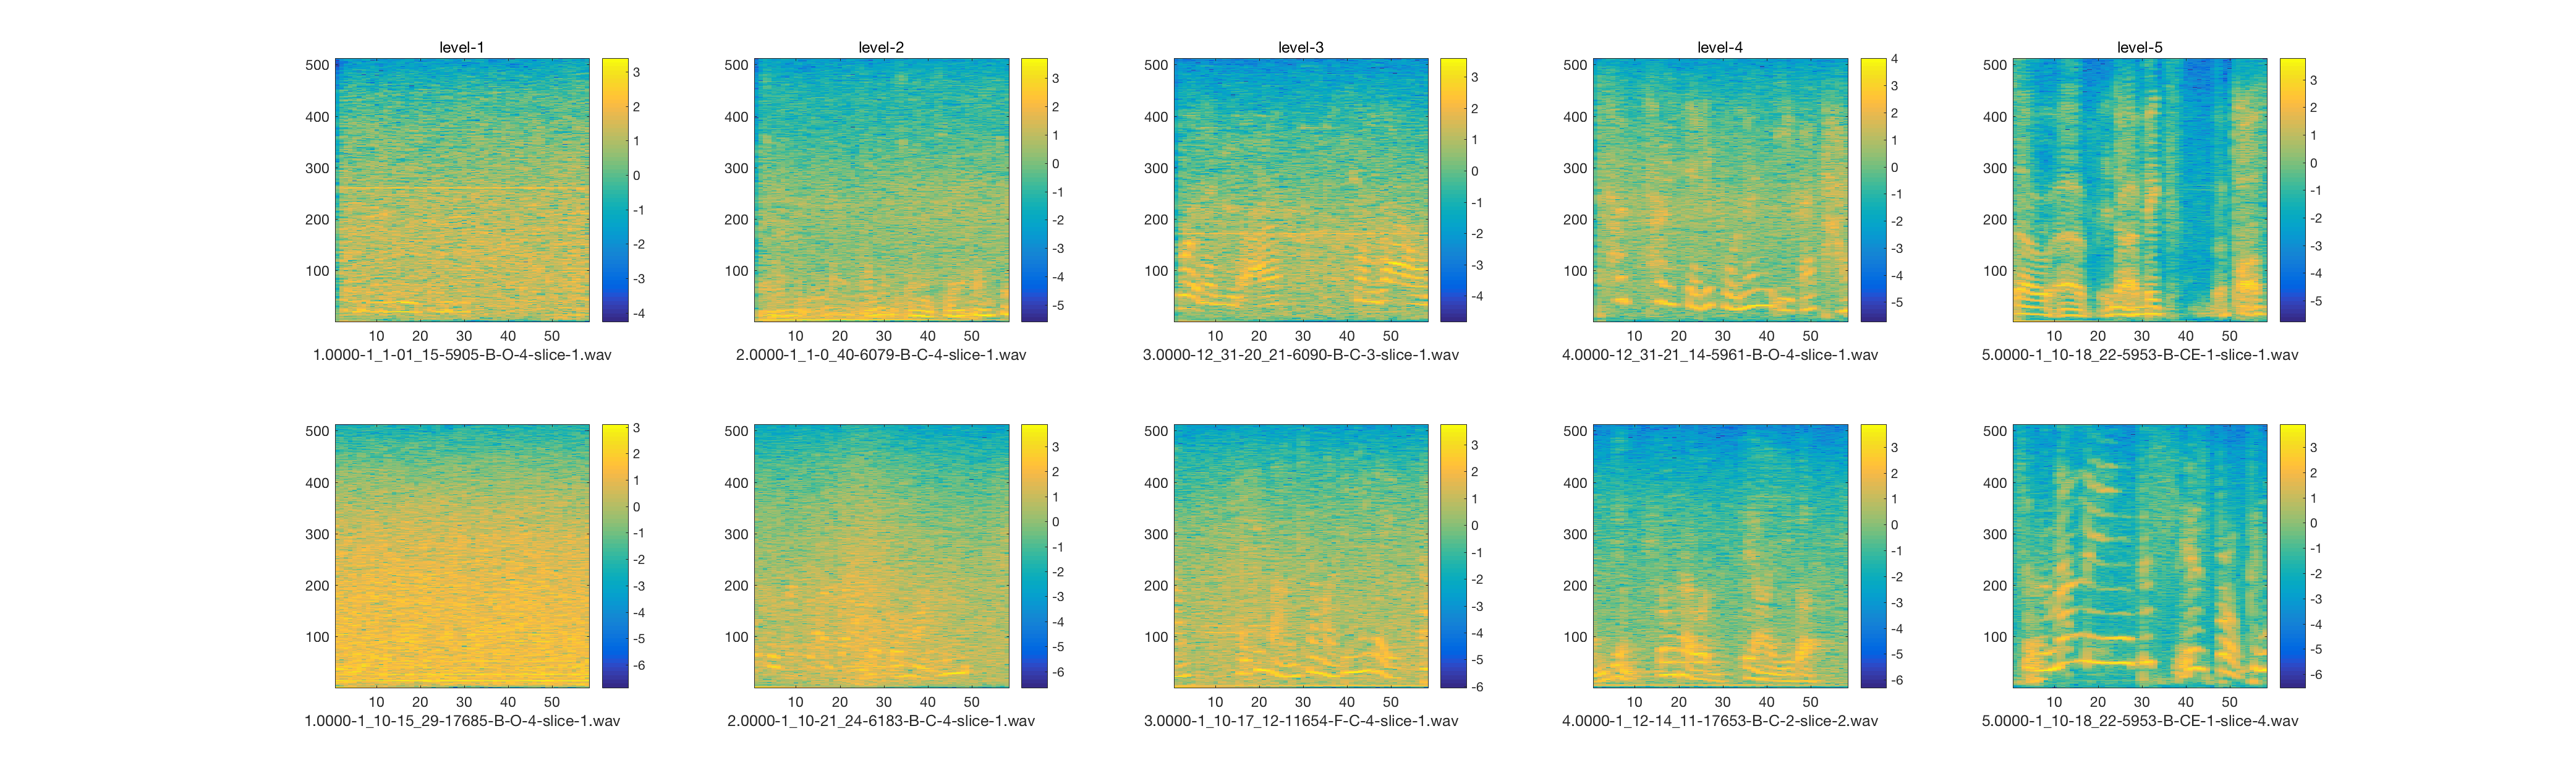
\includegraphics[width=1\textwidth]{timefreq}
\caption{不同质量的短波语音语谱图\label{fig:timefreq}}
\end{figure}

\begin{figure}
\centering
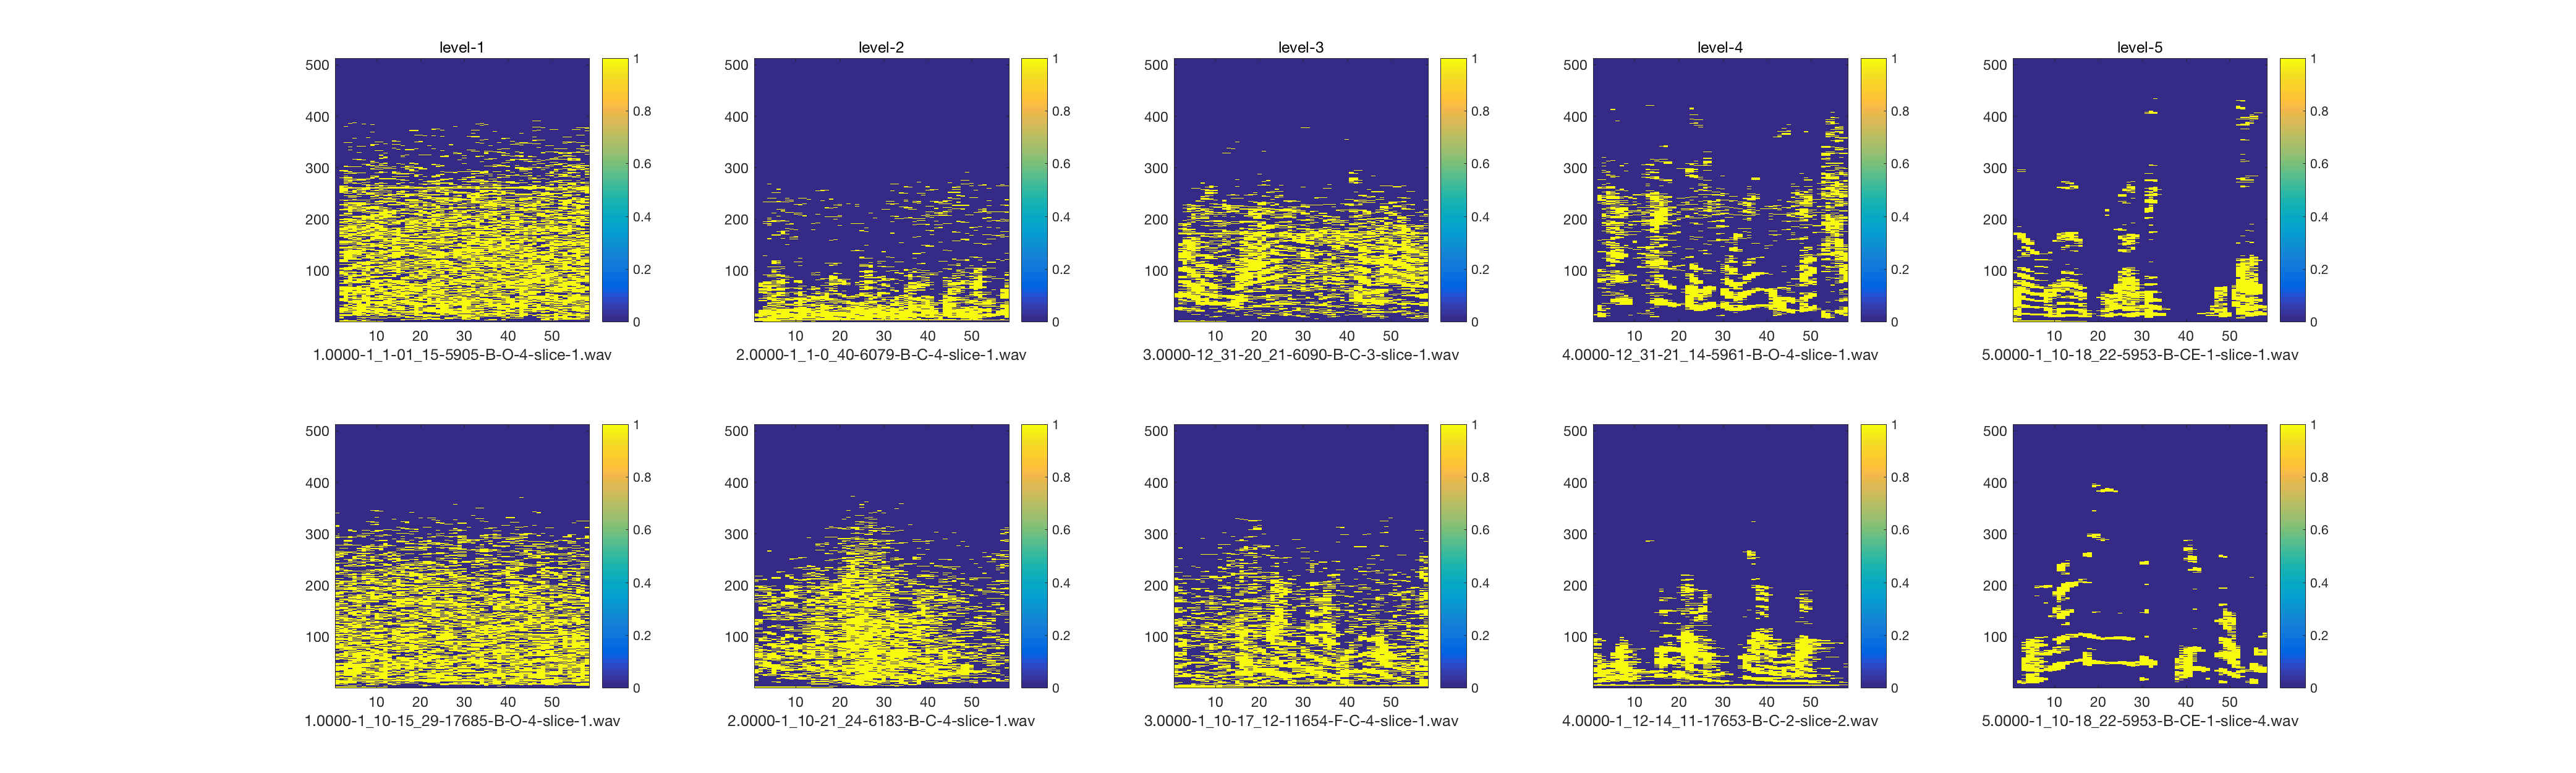
\includegraphics[width=1\textwidth]{timefreq-thr}
\caption{不同质量的短波语音二值化语谱图\label{fig:timefreq-thr0.3}}
\end{figure}

\begin{figure}
\centering
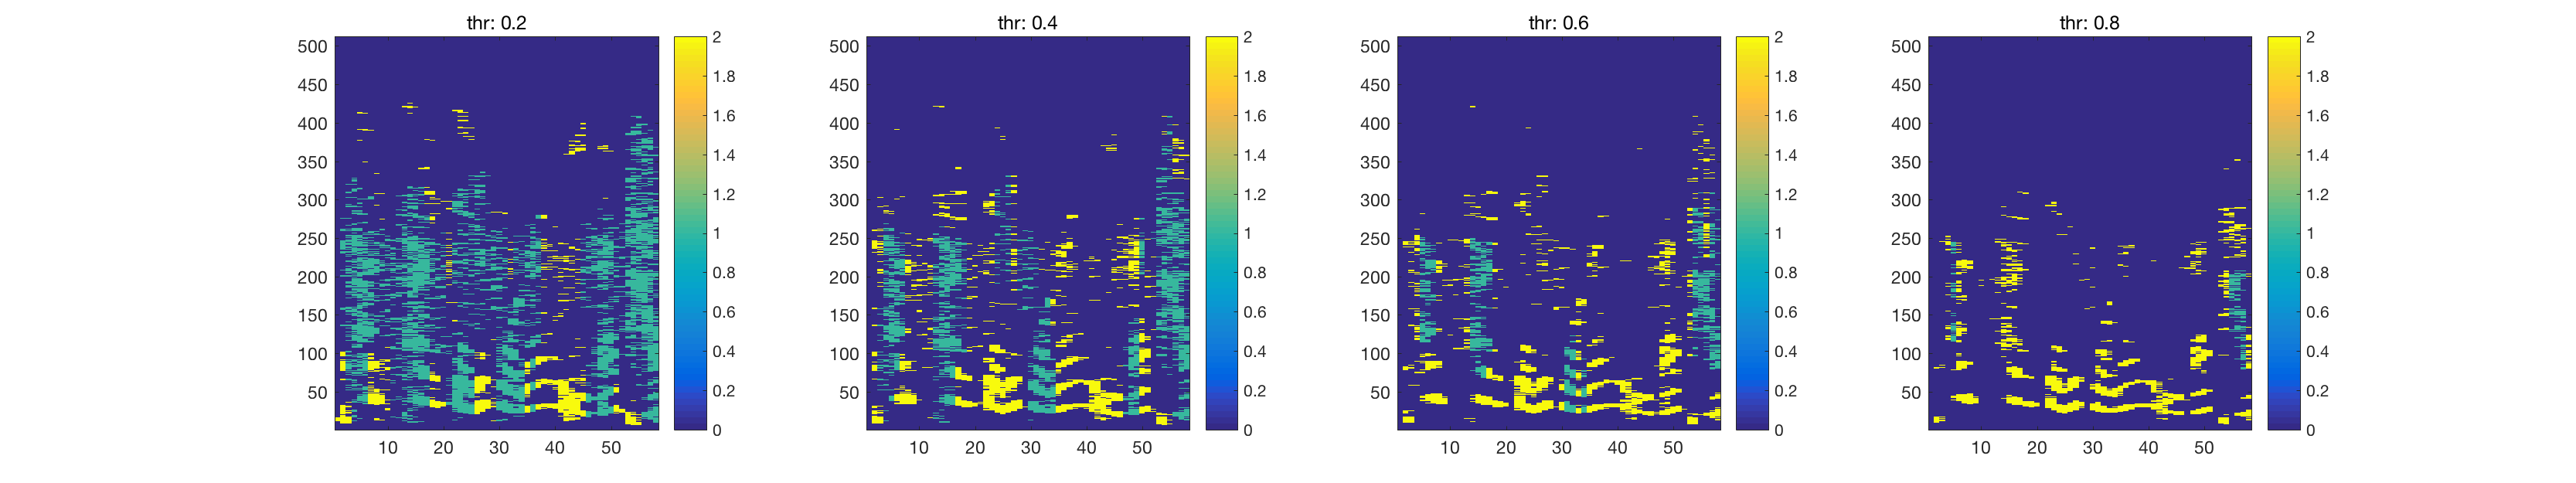
\includegraphics[width=1\textwidth]{timefreq-thrs-label}
\caption{不同阈值的二值化语谱图\label{fig:timefreq-thrs-label}}
\end{figure}

进一步地,从中选出一个语音信号,分别以0.2, 0.4, 0.6, 0.8为阈值绘制其二值化语谱图,如图~\ref{fig:timefreq-thrs-label}所示。而图中绿色区域是程序通过建立噪音模型,使用一些特征标注出的被噪音干扰的区域。可以发现,在阈值较低时,因为噪音部分留在了图上,所以看上去是大片大片的噪音;而当阈值逐渐升高,噪音部分逐渐从图上消失,留下的就都是纯净的语音信号。若当阈值超过某一阈值t时,语谱图上某一点不再被噪音干扰,那么这一点实际能量比t高出的部分就表征了这一点语音信号相对于噪音部分高出的强度。本文称之为该点的语音分辨率,计算语谱图上所有点的语音分辨率,进而得出语音质量的客观评价分。

\subsection{算法流程}

本小节介绍基于语谱图噪音模型的客观质量评价算法的具体流程,算法总体流程示意如图~\ref{fig:flowchart}所示。一维的短波语音信号经过加窗傅里叶变换得到二维的频域信号,其中横轴为时间维度,纵轴为频率维度。随后用不同阈值将语谱图转化成多张二值图像,再各个二值图像上使用图像处理的一些方法区分噪音区域和语音区域。再此基础上得到原始语谱图上各个点的“语音分辨率”,进而得到对于短波语音的客观评价分数。下面详细介绍各个步骤的内容。

\begin{figure}
\centering
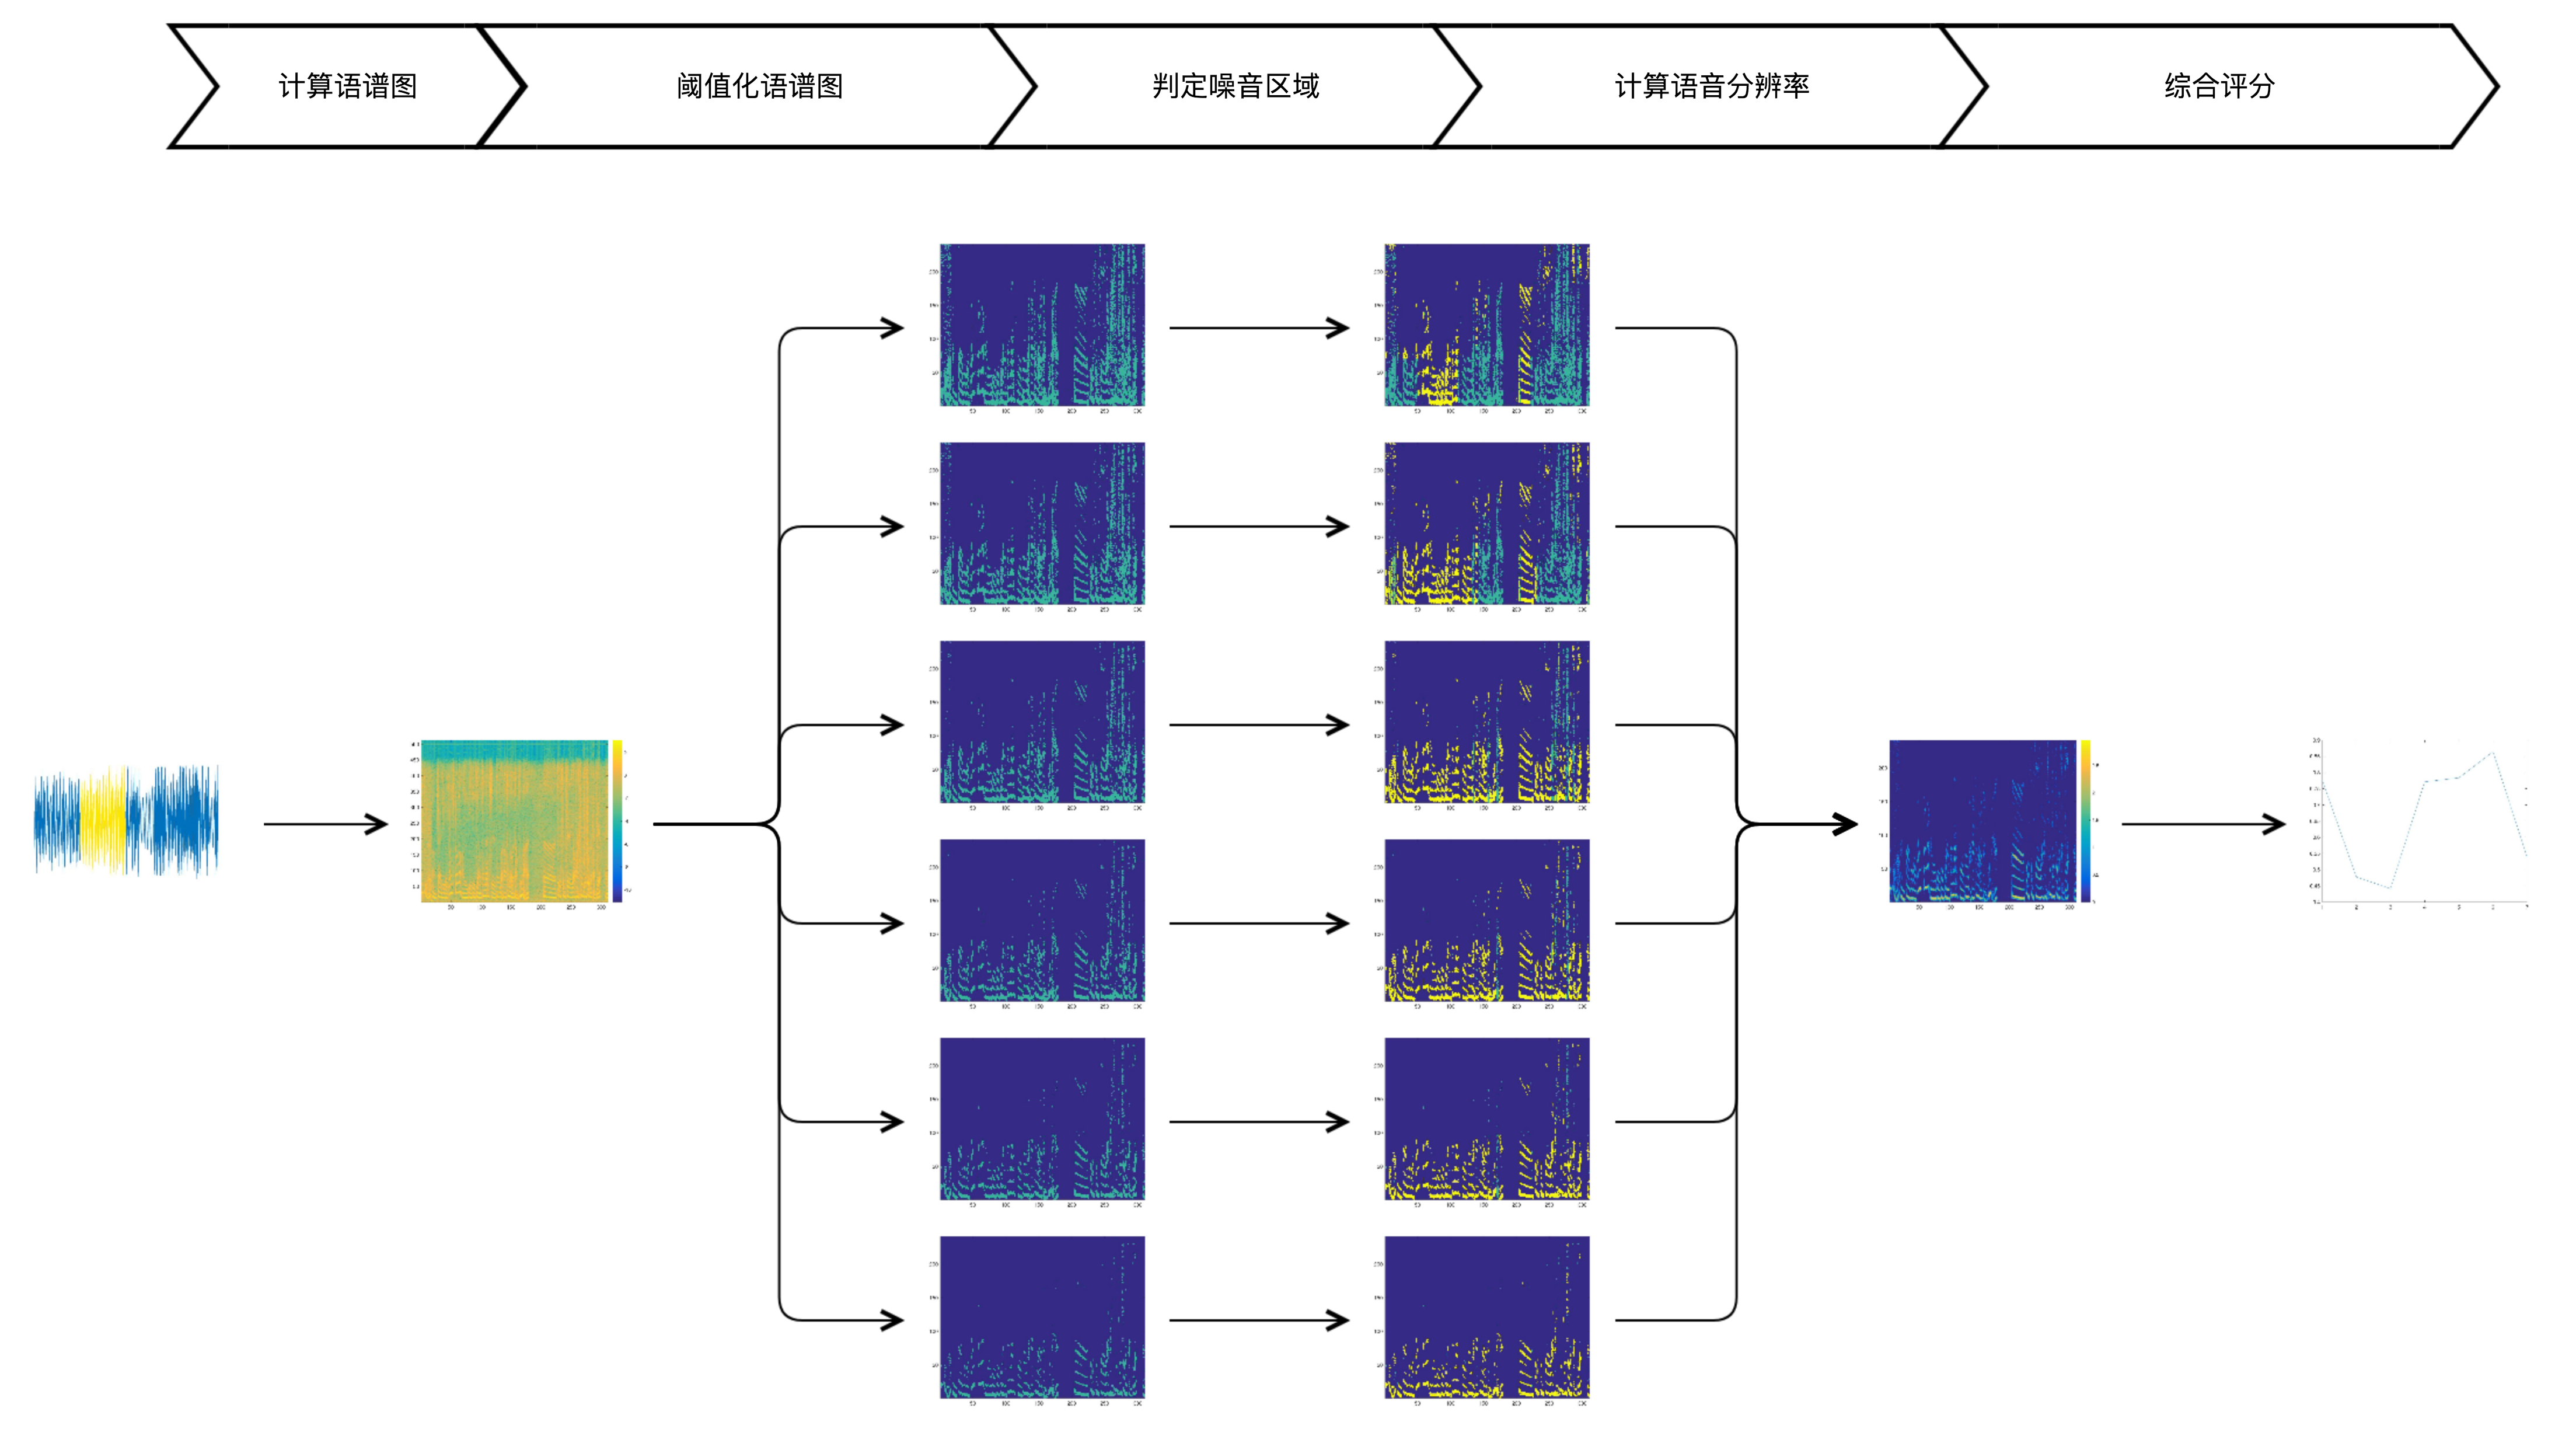
\includegraphics[width=0.8\textwidth]{flowchart}
\caption{基于语谱图噪音模型的客观质量评价算法流程\label{fig:flowchart}}
\end{figure}

首先根据上一小节介绍的语谱图的内容,使用短时傅里叶变换获得短波语音信号的语谱图$G(m,n)$。

取一系列的阈值$t_1<t_2<t_3<...<t_N$,我们进一步对语谱图做阈值化处理形成二值的语谱图,阈值化语谱图定义为

\begin{equation}\label{eq:thr_tf}
G_i(m, n) = \left\{
    \begin{array}{rcl}
    1, && {G(m,n)>t_i} \\
    0, && {G(m,n)\leq t_i}
    \end{array} \right.
\end{equation}

根据短波语音语谱图上的噪音模型,使用以下几种条件来判定噪音区域:
\begin{enumerate}
\item 区域$A_1$:语谱图上通过霍夫变换检测的与水平夹角小于1度的直线。
\item 区域$A_2$:某一长宽各大于一定阈值的范围内,$G_i(m,n)=1$的点数占据面积的80\%以上。
\item 区域$A_3$:某一连通域面积比上该连通域占据的宽度,其值超过一定阈值。
\item 区域$A_4$:某一连通域,其面积小于一定阈值。
\end{enumerate}

标注后的语谱图
\begin{equation}\label{eq:label_tf}
G_i^*(m, n) = \left\{
    \begin{array}{rcl}
    0, && {G_i(m,n)=0} \\
    1, && {G_i(m,n)=1且(m,n)\in \bigcup_{k=1}^4 A_k} \\
    2, && {else}
    \end{array} \right.
\end{equation}

定义集合
\begin{equation}\label{eq:collection}
\Psi(m,n)={i|G_i*(m,n)=2}
\end{equation}

定义语音分辨率
\begin{equation}\label{eq:resolution}
D(m,n) =  \left\{
    \begin{array}{rcl}
    0, && {\Psi(m,n)=\emptyset} \\
    G(m,n) - \min_{i\in\Psi(m,n)}t_i, && {\Psi(m,n)\neq\emptyset}
    \end{array} \right.
\end{equation}

对语音分辨率取平均得到客观评价分数
\begin{equation}\label{eq:score}
S = \frac{\sum D(m,n)}{\sum G_1(m,n)}
\end{equation}

为保证阈值化语谱图包含有效信息,阈值参数的取值范围应该是。一种简单的选取方法是直接在到选取$N$等分点。
为了尽量细致地刻画语谱图的特征,阈值的选取应该尽量密集,但同时算法的时间复杂度正比于阈值的数量,密集的阈值也会导致更高的计算复杂度。所以阈值的选取应当使用尽量少的阈值尽量高效地刻画语谱图的特征,上述选取方法显然不够高效。一方面,阈值很接近$\min{G(m,n)}$或者$\max{G(m,n)}$时,阈值化语谱图上的点非常少或者非常多,能提供的信息量很少。另一方面因为阈值增加同样大小,阈值化语谱图上的点数增加可能差异很大。均匀地选取阈值,会导致在有些区间,连续的几张阈值化语谱图过于相像而浪费计算资源,有些区间,阈值化语谱图又变化太快导致刻画不够细致。

一种改进的动态选取阈值的方法如下:先在5\%至20\%之间均匀选定一系列比例$\alpha_1,\alpha_2,\alpha_3,...,\alpha_N$,再计算得出对应的阈值$t_1,t_2,t_3,...,t_N$使得$\sum G_i(m,n)=\alpha_i M^2$。实验验证此种阈值选取方法要比前述方法效果提升很多。


\section{基于自编码器的客观质量评价算法}

上节介绍的基于语谱图噪音模型的客观质量评价算法虽然能够很好的评价短波语音的质量,实验也表明算法给出的评分能够反映人的主观感受。但是该算法是基于人为经验分析的语谱图噪音模型,在应用到其他领域的低信噪比语音时,由于可能存在的噪音不一样,需要重新分析噪音的模型特征。所以该算法针对性很强,而适用性则较窄,迁移应用较难。

为此,本节从另一个角度出发,通过人工神经网络的自编码器学习纯净短波语音的语谱特征,对语音部分而非噪音部分建模,然后再使用自编码器来评价短波语音的质量。由于人工神经网络的学习可以自动完成,不需要过多人工干预,所以这种方法可以方便的迁移到其他领域的应用中。

\subsection{梅尔频谱语谱图}

~\ref{section:alg1-1}小节中介绍的语谱图在应用到自编码器中时,频率方向采样太密,使得输入向量长度太长,所以我们希望对频率方向降采样。由于人耳的听觉特性在频率方向并非线性,人耳在低频区域有更多的感受器,对频率的分辨相对灵敏,而随着频率升高,对频率的分辨逐渐降低。所以降采样时我们使用根据这种人耳听觉特性而设计的非线性的滤波器组——梅尔滤波器组。

梅尔滤波器组来源于语音信号处理中常用的梅尔频率倒谱系数(MFCC)的计算过程。滤波器数量我们设定为40,使用40个三角滤波器$H_k, k=0,1,2...,39$组成的滤波器组来处理原始语谱图。每个滤波器的输出对应于一个频带的能量,40个频带的中心频率分布是非线性的,在低频处分布较密集,高频处分布较疏松。每个滤波器中心频率和$k$的关系为~\ref{eq:mel-freq},各个滤波器的冲击响应$H_k$满足~\ref{eq:mel-filters}。

\begin{equation}\label{eq:mel-freq}
f(k) = 700(10^{k/2595}-1)
\end{equation}

\begin{equation}\label{eq:mel-filters}
H_k(n) = \left\{
    \begin{array}{rcl}
    0, && {n<f(k-1)} \\
    \frac{n-f(k-1)}{f(k)-f(k-1)}, && {f(k-1)\leq n < f(k)} \\
    1, && {n=f(k)} \\
    \frac{f(k+1)-n}{f(k+1)-f(k)}, && {f(k) < n \leq f(k+1)} \\
    0, && {n > f(k+1)}
    \end{array} \right.
\end{equation}

使用这40个三角滤波器组成的梅尔滤波器组,我们得到更符合人耳听觉特性的梅尔频谱(Mel-Frequency)语谱图M(m, k),其中$m=0,1,2,...M-1; k=0,1,2,…39$。

\subsection{自编码器结构}

由于语音存在一定的结构特征,所以语音频谱中存在冗余信息,可以通过更少的信息来表示。人工神经网络构建的自编码器(Autoencoder),可以用来提取高维向量中的结构化特征,将其压缩到较低维空间表示。
对8kHz的短波语音使用32ms的窗长加汉明窗,以16ms的长度移动汉明窗,使用40个梅尔频谱滤波器,生成梅尔频谱语谱图。取连续7帧语音的语谱图,拼接成自编码器的输入向量,向量长度为7*40 = 280。自编码器的隐藏层大小设置为80,网络结构如图~\ref{fig:autoencoder}所示。

\begin{figure}
\centering
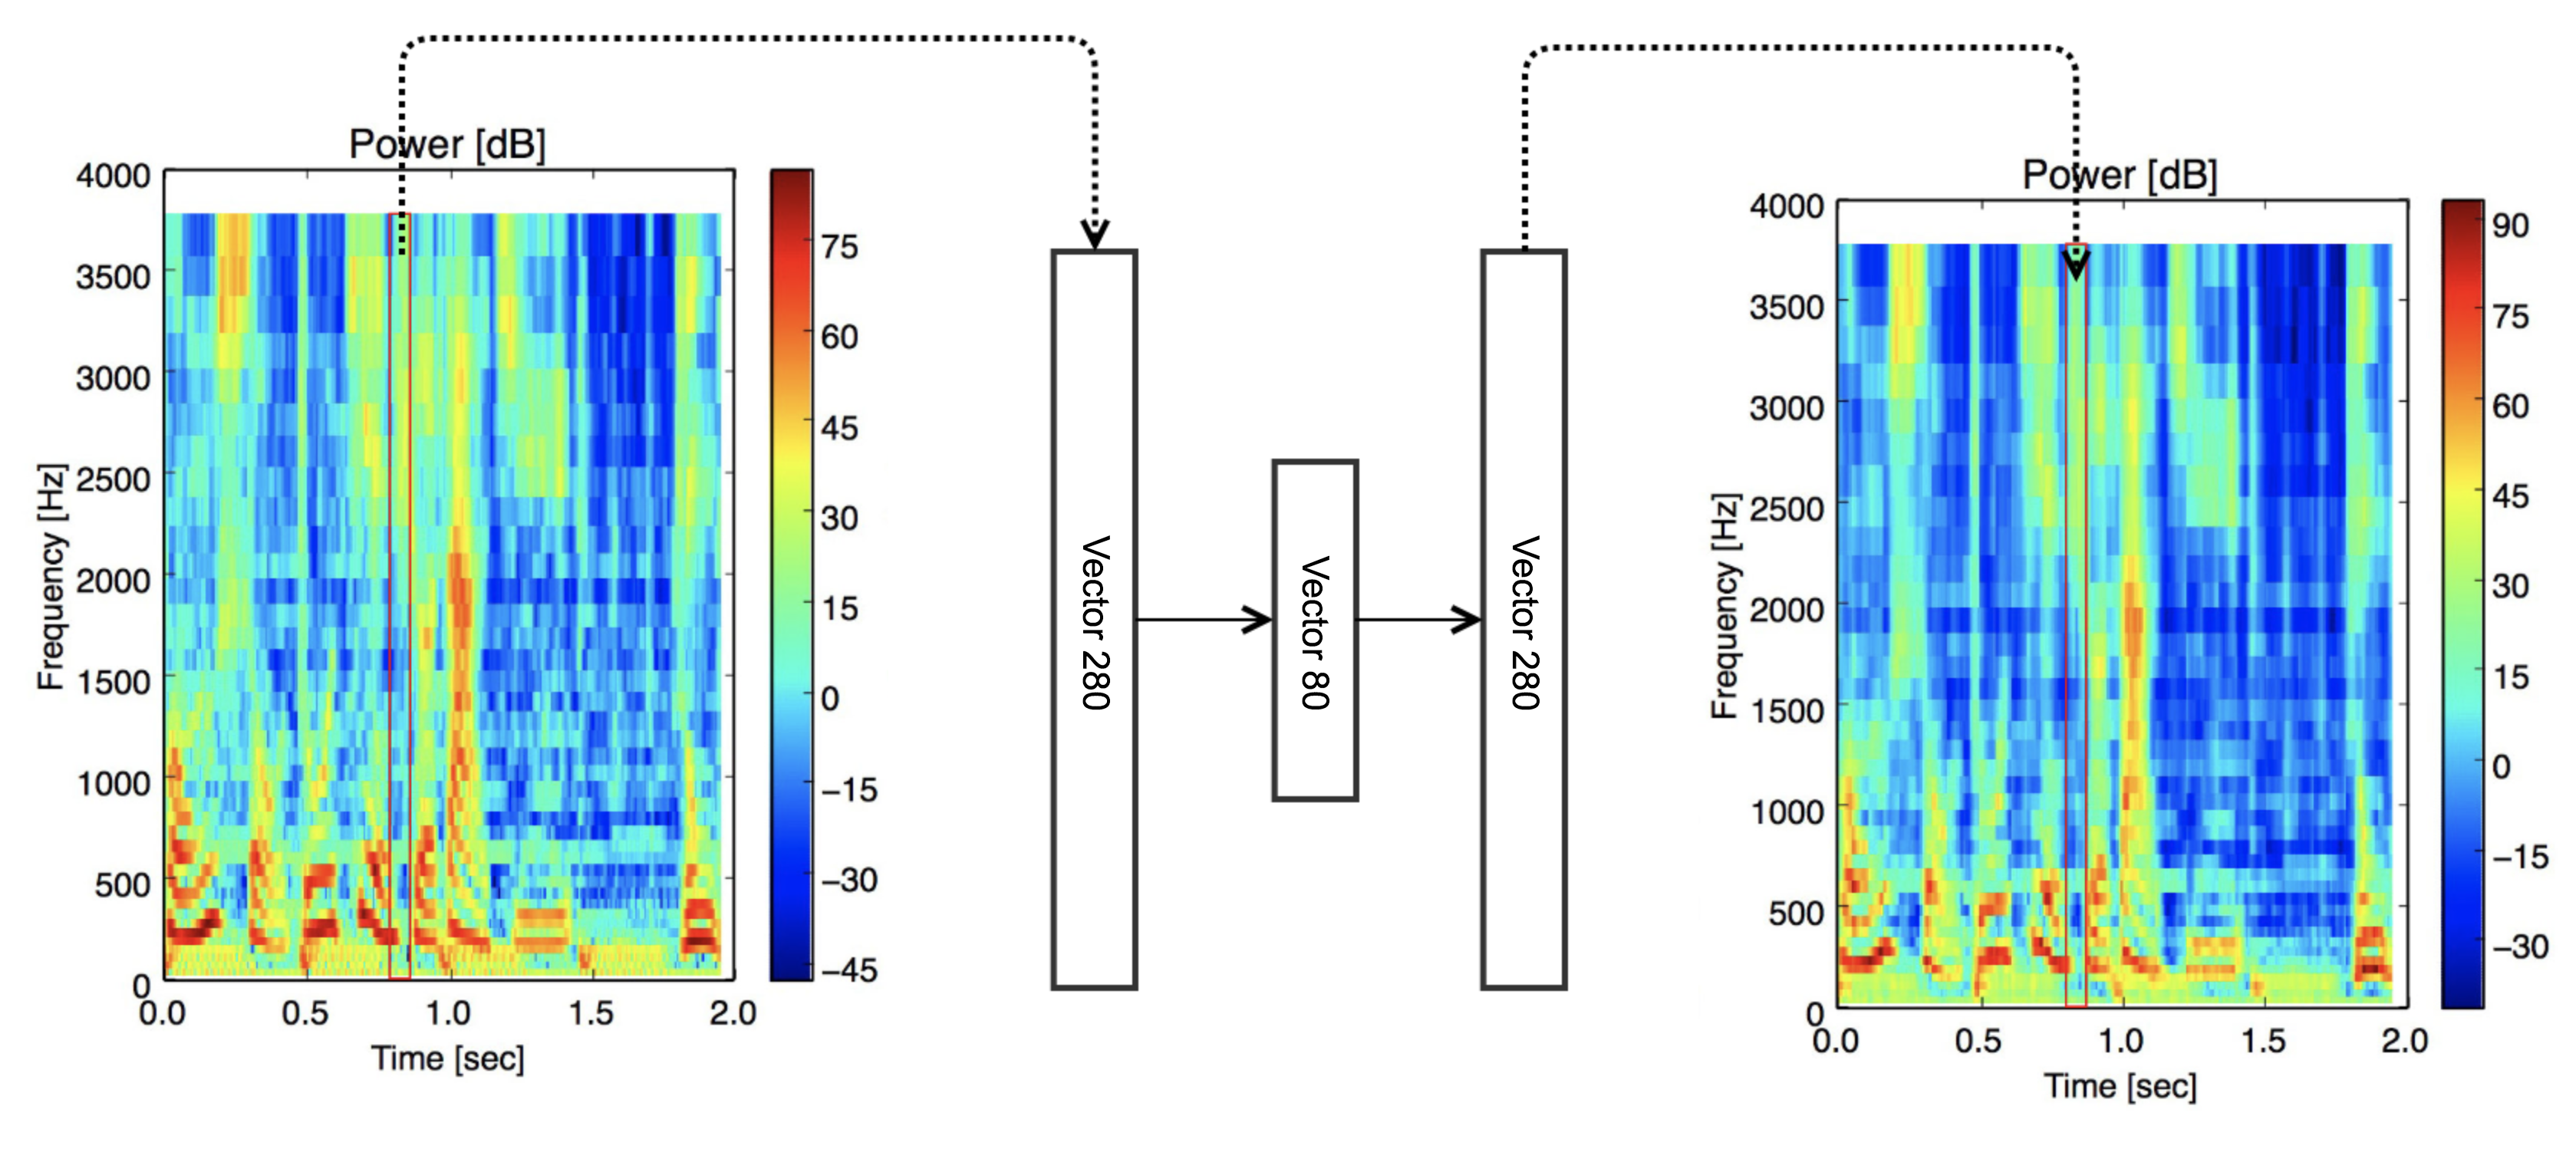
\includegraphics[width=0.8\textwidth]{autoencoder}
\caption{自编码器网络结构\label{fig:autoencoder}}
\end{figure}

自编码器网络使用tensorflow\cite{abadi2016tensorflow}实现,隐藏层激活函数使用softplus函数$\sigma(x)=ln⁡(e^x+1)$,使用质量非常高、基本未受到干扰或者噪音污染的短波语音训练自编码器,使其学习短波语音的语谱结构特征。使用总计时长约5小时的清晰短波语音进行训练,每个训练样本的语音时长为16*8=128ms,故总计样本数量为14万左右。训练的batch大小设置为256,初始学习速率0.001。
经过一段时间的训练,自编码器可以学习到清晰短波语音的语谱特征,如图~\ref{fig:ae-pure1}是一段清晰短波语音经过自编码器的输入输出结果。可以看出,尽管自编码器将输入向量的长度由输入的280压缩到了隐藏层的80,最终输入和输出的梅尔语谱图相差甚微,基本的特征都得到了保留。

\begin{figure}
\centering
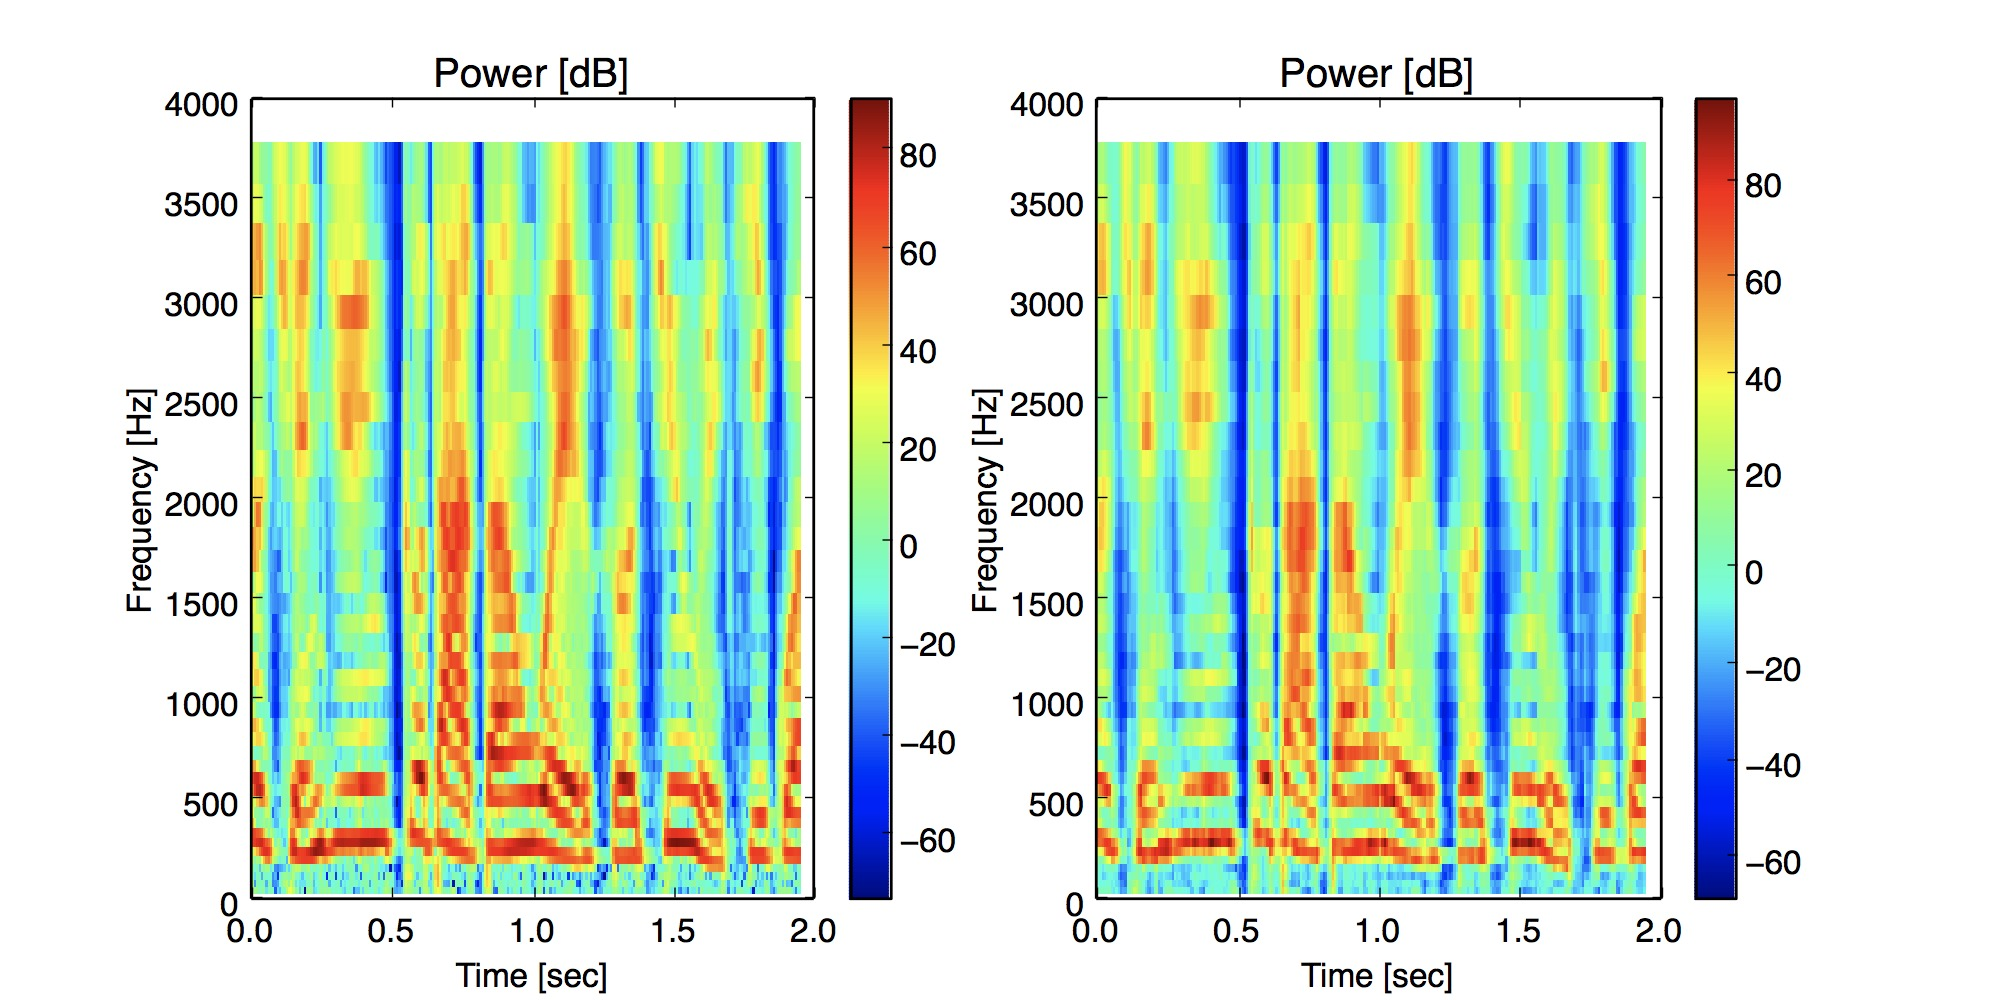
\includegraphics[width=0.8\textwidth]{ae-pure1}
\caption{自编码器输入输出语谱图(清晰语音)\label{fig:ae-pure1}}
\end{figure}

% \chapter{果蝇活动台提取}
\label{chapter:container_split}

果蝇活动台提取步骤的输入包含多个果蝇活动台的视频,输出多个子视频,每个子视频均包含单独的果蝇活动台,为后续的果蝇行为分析做准备。果蝇行为视频的拍摄环境差异较大,用现有算法流程可能需要针对每个拍摄环境单独选择算法参数,为此本章在形状检测算法的基础上,提出了一种自适应的果蝇活动台提取算法。此外,现有的果蝇活动台提取算法往往存在较大的误差。为此,本文利用果蝇活动台之间固有的排列模式,提出了一种基于特定排列的果蝇活动台提取算法,提高果蝇活动台提取算法的准确性。

\section{活动台提取算法}\label{sec:container_split}

果蝇活动台一般是标准的圆形,分布在背景相对简单的拍摄场景中,可以根据活动台的形状进行提取。目前常见的果蝇活动台提取的标准算法流程一般包括:

\begin{enumerate}
\item 从视频中抽取$M$帧 $I_{k_1}, I_{k_2}, \ldots, I_{k_M}$,其中$M$的取值一般在$100\sim 1000$之间,$k_1, k_2, \ldots, k_M$表示视频帧的序号。为了尽可能的覆盖整个视频时长,对于$N$帧的视频,$k_1, k_2, \ldots, k_M$ 一般选取为$0\sim N$的等差数列,或者$0\sim N$中无放回的M次随机抽样;
\item \label{hough_step} 利用边缘检测算法得到$I_{k_1}, I_{k_2}, \ldots, I_{k_M}$的边缘,进而利用圆检测算法,找到视频帧$I_{k_1}, I_{k_2}, \ldots, I_{k_M}$中的圆。边缘检测算法可以选用Canny算子\cite{canny1986computational},圆检测算法可以选取Hough圆检测算法\cite{hough_circle_1990};
\item \label{container_center_step}对上一步骤中检测得到的圆的中心点坐标进行聚类,得到坐标中心的位置,即为活动台的位置。聚类中心的数目应等于果蝇活动台的数目。
\item \label{container_radius_step} 对\ref{hough_step}步骤中得到的圆的大小进行聚类,得到活动台的大小。因为果蝇活动台的构造一般包含2个圆,其中外侧圆限制了果蝇活动的范围,中心还有一个圆形凹槽用于投放果蝇食物,因而需要用聚类算法分别找到2个圆的大小。聚类中心的数目设置为每个果蝇活动台俯视图中圆形的数目;
\item \label{container_timeline_search}根据果蝇活动台的位置和中心,在原始视频中利用二分查找法,找到果蝇放入和移出视频的时间;
\item 利用\ref{container_center_step}, \ref{container_radius_step}, \ref{container_timeline_search} 的结果,逐帧对原视频进行切割,得到$M$个子视频。
\end{enumerate}

上述步骤涵盖了完整的果蝇活动台提取流程,其中,\ref{hough_step}步骤是关键步骤,Hough圆检测算法的结果决定了算法的准确性。但经验表明,果蝇活动台的边缘往往存在部分厚度或者阴影,利用Hough圆检测算法往往很难得到精确的解。为了使Hough圆检测算法找到数量足够、位置精确的圆,需要对算法参数加以优化。

Hough圆检测算法一般分为2步:首先对输入图像进行Canny边缘检测,其中参数$param_1$用于控制Canny算子的敏感度,$param_1$越小,对边缘越敏感;然后对图像进行Hough变换,得到参数空间中每个点对应图像空间中像素点的个数。为了减小参数空间的范围,可以设定半径的取值区间$[R_{min}, R_{max}]$;最后在特征空间中选取对应特征点数目超过$param_2$的极大值点作为检测结果,$param_2$参数值越小,检测到的圆的数目越多。随着$param_1$和$param_2$的减小,算法的对计算资源和内存资源的要求可能会急剧增加,此外,过低的$param_1$和$param_2$也有可能将更多的噪声信息误判为圆,从而影响到检测的准确性。

综上可知,可以通过调整活动台半径的范围$[R_{min}, R_{max}]$、$param_1$和$param_2$优化Hough圆检测的结果。活动台半径可以通过对视频分辨率和视频中摆放的活动台数目进行估算,也可以通过其他方式手动测量,在相同的拍摄环境下,果蝇活动台在视频中的尺寸是基本一致的,$[R_{min}, R_{max}]$也不需要重复配置。

$param_1$和$param_2$的设置可以通过自适应过程加以调整。首先,通过设置较大的$param_1$和$param_2$,对视频帧进行Hough圆检测,如果检测到的圆的数目和果蝇活动台的实际数目满足一定的条件,则认为找到了合适的$param_1$和$param_2$;否则,减小$param_1$和$param_2$,直到满足特定的条件为止。因为Hough算法的计算复杂度较高,在处理分辨率相对较高的输入视频时速度较慢,因而在对参数$param_1$和$param_2$进行自适应时,为了进一步降低计算复杂度,提高程序运行的效率,可以进一步降低对视频帧的采样数目,一般选取$30\sim 100$帧即可。

完整的果蝇活动台提取算法如算法~\ref{alg:container_split_adaptive}所示。
\begin{algorithm}
    \caption{自适应的活动台检测算法}
    \label{alg:container_split_adaptive}
\begin{algorithmic}[1]
\INPUT
    \Statex 果蝇行为视频;
    \Statex 活动台的数量$K_1$;
    \Statex 活动台圆的数量$K_2$;
    \Statex 活动台的最大可能半径$R_{max}$ 和 最小可能半径 $R_{min}$;
    \Statex Hough圆检测参数最大自适应次数$max\_iters$。
\OUTPUT
    \Statex 活动台的圆心$(x_1, y_1), \ldots, (x_{K_1},y_{K_1})$;
    \Statex 活动台的外径$R$;
    \Statex 活动台的移入时刻$t_{1, in}, \ldots, t_{K_1, in}$和移出时刻$t_{1, out}, \ldots, t_{K_1, out}$;
\State 从视频中抽取$M_1$帧视频$\{ I_{k_1}, I_{k_2}, \ldots, I_{k_{M_1}} \}$;
\State 初始化Hough圆检测的参数 $param_1^{\{0\}} = 200$, $param_2^{\{0\}} = 200$;
\For {$i = 0$ to $max\_iters$;}
    \State 对视频帧$\{ I_{k_1}, I_{k_2}, \ldots, I_{k_{M_1}} \}$,使用参数$param^{\{i\}}_1$和$param^{\{i\}}_2$进行Hough圆变换检测,得到$N_i$个圆;
    \If {$N_i < 3K_1$; }
        \State $param_1^{\{i+1\}} = 0.9\times param_1^{\{i\}}, param_2^{\{i+1\}} = 0.9\times param_2^{\{i\}}$
    \Else
        \State break
    \EndIf
\EndFor
\State 从视频中抽取$M_2$帧视频$\{ I_{l_1}, I_{l_2}, \ldots, I_{l_{M_2}} \}$
\State 使用参数$param_1 = param_1^{\{i\}}, param_2 = param_2^{\{i\}}$,利用Hough圆检测算法,对视频帧$\{ I_{l_1}, I_{l_2}, \ldots, I_{l_{M_2}} \}$进行圆检测,得到$N$个圆 $(\tilde{x}_1, \tilde{y}_1, r_1), \ldots, (\tilde{x}_N, \tilde{y}_N, r_N)$;
\State 使用GMM算法\cite{GMM_1999}将圆心$(\tilde{x}_1, \tilde{y}_1), \ldots, (\tilde{x}_N, \tilde{y}_N)$聚为$K_1$类,得到$(x_1, y_1), \ldots, (x_{K_1},y_{K_1})$;\label{alg:arena:clusterXY}
\State 使用GMM算法将半径$r_1, \ldots, r_N$聚为$K_2$类,得到$R_1, R_2, \ldots, R_{k_2}$,最终活动台的外径为$R = \max(R_1, R_2, \ldots, R_{k_2})$;\label{alg:arena:clusterR}
\State 检测$(x_i, y_i)$周围检测到的Hough圆的数目,利用二分查找法,分别查找$K_1$个聚类中心的移入视频的时刻$t_{i,in}$和移出视频的时刻$t_{i, out}$;
\State 输出$(x_1, y_1),\ldots,(x_K, y_K)$、$R$和$t_{1, in}, \ldots, t_{K_1, in}$以及移出时刻$t_{1, out}, \ldots, t_{K_1, out}$。
\end{algorithmic}
\end{algorithm}

通过自适应,可以提高果蝇活动台提取算法的鲁棒性,减少果蝇活动台提取步骤中的手工操作步骤。

\section{基于特定排列的果蝇活动台提取算法} \label{sec:container_split_fixed_array}

果蝇活动台提取算法的关键步骤在于Hough圆检测,而Hough圆检测算法的精确度往往比较差。为此可以依据果蝇活动台的排列情况,进一步校正活动台的位置。

在部分实验环境下,果蝇活动台被放置在特定的模具中,按照固定的方式排列,如图~\ref{fig:containers_fixed_by_array}所示。图~\ref{fig:containers_fixed_by_array}中,果蝇活动台呈矩形排列。利用果蝇活动台之间的位置信息,可以进一步提高果蝇活动台提取的准确性。一般来说,为了提高果蝇活动台的排列密度,果蝇活动台通常 按照矩形或正六边形进行排列,上述两种排列都很容易处理,下面仅以矩形排列为例,说明如何利用活动台的排列信息提高活动台提取的准确性。

\begin{figure}[htb]
\centering
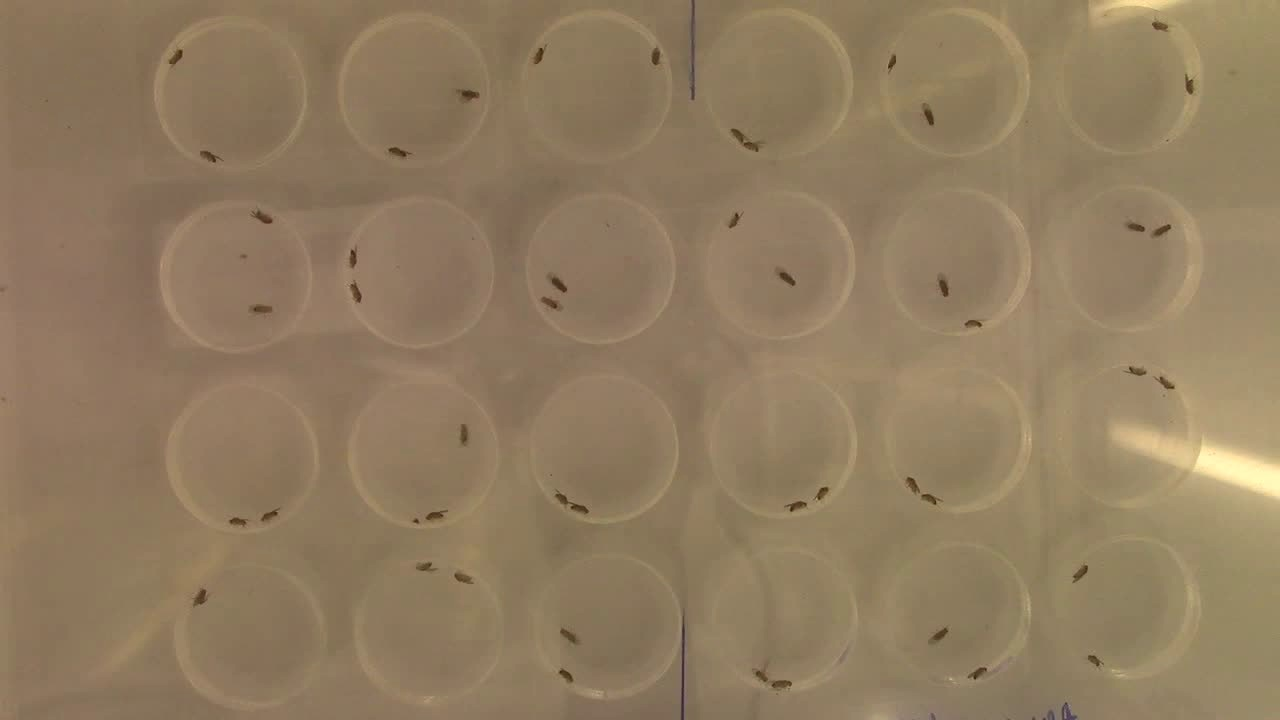
\includegraphics[width=0.8\textwidth]{containers_fixed_by_array}
\caption{按照矩形模式排列的果蝇活动台}
\label{fig:containers_fixed_by_array}
\end{figure}

在某些拍摄条件下,果蝇活动台的视频中存在较大的噪声,如图~\ref{fig:containers_fixed_by_array}所示,整个视频中的光照条件并不一致,图像的左侧亮度明显暗于右侧,整幅图中存在明显的阴影,右侧甚至存在清晰、明亮的光照情况,此外,果蝇活动台的侧壁也明显存在一定的模糊现象。上面的各种问题在多个拍摄场景中都有体现,尤其是果蝇活动台的边缘模糊,给Hough圆检测算法带来很大的影响,使得部分圆难以被准确检测到。此外,对检测到的圆心直接进行聚类时,受到噪声圆或聚类中心初始化的影响,聚类结果可能会有问题,使得部分活动台中心周围有不止一个聚类中心。利用果蝇活动台之间的排列关系可以一定程度上解决上述问题。下面介绍算法的具体过程。

首先,利用第\ref{sec:container_split}节中的自适应果蝇活动台提取算法,提取视频中果蝇活动台的大致位置,得到$K_1$个果蝇活动台中心$(x_1,y_1), \ldots, (x_{K_1},y_{K_1})$。

其次,根据果蝇活动台的排列方式,确定实际果蝇活动台在理想坐标系下的坐标$(\hat{x}_1, \hat{y}_1), (\hat{x}_2, \hat{y}_2), \ldots, (\hat{x}_{K_1}, \hat{y}_{K_1})$。当果蝇活动台按照图~\ref{fig:containers_fixed_by_array}所示进行排列时,在理想坐标系下,编号为$i$的果蝇活动台中心的位置为$(m_i, n_i)$,$m_i$和$n_i$分别表示该果蝇活动台所在的行数和列数。

再次,建立图像坐标系中坐标$(x_1,y_1),\ldots,(x_K,y_K)$和理想坐标系中坐标$(\hat{x}_1, \hat{y}_1), (\hat{x}_2, \hat{y}_2), \ldots, (\hat{x}_{K_1}, \hat{y}_{K_1})$之间的一一对应关系。首先,找到聚类中心的最小外包矩形;然后,将外包矩形旋转到某一边和坐标轴方向平行,并求出每个坐标方向上格点的距离;最后,根据每个格点的坐标,计算对应的行和列的位置,得到在理想坐标系下的坐标。在实际场景中,果蝇活动台的摆放方向和坐标轴基本平行时,可以省略上述求解外包矩形并旋转的步骤。

然后,建立从$(x_1, y_1),\ldots,(x_K, y_K)$到$(\hat{x}_1, \hat{y}_1), (\hat{x}_2, \hat{y}_2), \ldots, (\hat{x}_{K_1}, \hat{y}_{K_1})$的仿射变换。记仿射变换为$A$:
$$
A = \begin{bmatrix}
    a_{11} & a_{12} & a_{13} \\
    a_{21} & a_{22} & a_{23}
  \end{bmatrix}.
$$

根据映射关系,得到式(\ref{eq:img2ideal}):
\begin{equation} \label{eq:img2ideal}
\begin{bmatrix}
    a_{11} & a_{12} & a_{13} \\
    a_{21} & a_{22} & a_{23}
  \end{bmatrix}
\begin{bmatrix}
    x_{1} & x_2 & \ldots & x_K\\
    y_{1} & y_2 & \ldots & y_K\\
    1 & 1 & \ldots & 1
\end{bmatrix} =
\begin{bmatrix}
    \hat{x}_{1} & \hat{x}_{2} & \ldots & \hat{x}_K\\
    \hat{y}_{1} & \hat{y}_{2} & \ldots & \hat{y}_K
\end{bmatrix}.
\end{equation}

式(\ref{eq:img2ideal})共包含6个未知数,理论上需要3组坐标点即可求解。正常情况下,果蝇活动台的数目会超过3个,可以用最小二乘法求解式(\ref{eq:img2ideal})。为了便于表示,记
\begin{flalign}
P &= \begin{bmatrix}
    x_{1} & x_2 & \ldots & x_K\\
    y_{1} & y_2 & \ldots & y_K\\
    1 & 1 & \ldots & 1
\end{bmatrix}, \\
Q &= \begin{bmatrix}
    \hat{x}_{1} & \hat{x}_{2} & \ldots & \hat{x}_K\\
    \hat{y}_{1} & \hat{y}_{2} & \ldots & \hat{y}_K
\end{bmatrix},
\end{flalign}
得到$AP=Q$。根据最小二乘法,得到$A$的表达式:
\begin{equation}
A = QP^T(PP^T)^{-1}.
\end{equation}

最后,求解仿射变换$A$的逆变换$B$,即$B$变换将坐标从理想坐标系映射回图像坐标系,得到活动台的准确位置:
\begin{equation}
P' = BQ,
\end{equation}
其中
\begin{equation}
P' = \begin{bmatrix}
    \bar{x}_{1} & \bar{x}_{2} & \ldots & \bar{x}_{K_1} \\
    \bar{y}_{1} & \bar{y}_{2} & \ldots & \bar{y}_{K_1}
\end{bmatrix}.
\end{equation}

得到果蝇活动台准确的位置$(\bar{x}_1, \bar{y}_1), (\bar{x}_2, \bar{y}_2), \ldots, (\bar{x}_{K_1}, \bar{y}_{K_1})$后,对视频进行二分查找,得到果蝇活动台放入和移出的时刻,最后,根据果蝇活动台的位置、大小、放入时刻、移出时刻,对原始视频进行切割,得到单独的果蝇活动台视频。

果蝇视频的文件体积较大,一般需要对视频进行压缩。对于一个分辨率为1920$\times$1080、帧率为25帧的果蝇行为视频,完全无压缩的10分钟视频文件大小为84G,这就要求对果蝇行为视频采用适当的压缩。因为果蝇的身体尺寸较小,且果蝇的翅膀呈现半透明的特点,很容易因为视频压缩而损失视频信息。本文没有分析视频编码对果蝇行为分析结果带来的影响,所有的果蝇视频,包括原始输入视频和中间结果视频,均被保存为MPEG2-4格式。为了进一步提高果蝇行为识别的精度,可能需要进一步研究视频编码的影响。

\tikzstyle{block} = [rectangle, draw, text width=18em,  text centered, rounded corners, minimum height=3.5em]
\tikzstyle{arrow} = [thick, draw, -latex']

\begin{figure}[htb]
\centering
% 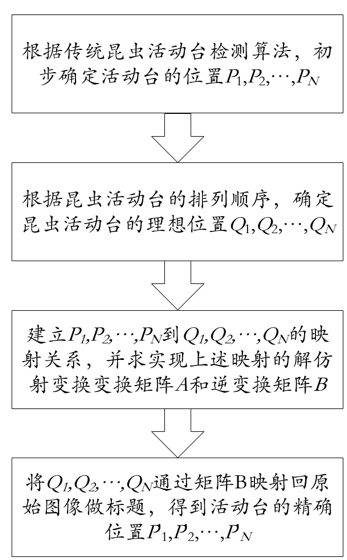
\includegraphics[scale=0.95]{fix_array_container_split}

\begin{tikzpicture}[node distance=2.5cm]

\node [block, minimum height=7em] (init) {\heiti 根据传统果蝇活动台检测算法,初步确定活动台的位置$P_1, P_2, \ldots, P_N$};
\node [block, below = 0.5cm of init, minimum height=7em] (idea_position) {\heiti 根据果蝇活动台的排列,确定果蝇活动台在理想坐标系下的位置$Q_1, Q_2, \ldots, Q_N$};
\node [block, below = 0.5cm of idea_position, minimum height=7em] (transform) {\heiti 建立$P_1, P_2, \ldots, P_N$到$Q_1, Q_2, \ldots, Q_N$的映射关系,并求解映射变换矩阵$A$和逆变换矩阵$B$};
\node [block, below = 0.5cm of transform, minimum height=7em] (inv_trans) {\heiti 将$Q_1, Q_2, \ldots, Q_N$通过变换$B$映射回原图像坐标系,得到活动台的精确位置$P'_1, P'_2, \ldots, P'_N$};

\path [arrow] (init) -- (idea_position);
\path [arrow] (idea_position) -- (transform);
\path [arrow] (transform) -- (inv_trans);

\end{tikzpicture}
\caption{基于特定排列的果蝇活动台提取算法流程}
\label{fig:fix_array_container_split_procedure}
\end{figure}

\section{果蝇活动台分割结果}

针对如图~\ref{fig:containers_fixed_by_array}所示的果蝇活动台,设置参数 $K_1 = 24, K_2 = 1, R_{max} = 80, R_{min} = 30, max\_iters = 15$,进行果蝇活动台提取。

首先对视频进行30帧采样,估算合适的$param_1$和$param_2$;然后,选取300帧视频进行Hough圆检测,如图~\ref{fig:simple_hough_circle}所示。从300帧视频中共计检测出了19658个圆,为了便于展示,在图~\ref{fig:simple_hough_circle}中仅包含随机抽取的394个圆。从图~\ref{fig:simple_hough_circle}中可以看出,Hough圆检测算法可以比较准确的找到活动台。但因为视频中存在不同的亮度等条件,造成圆检测结果的空间分布存在明显的不平衡,部分活动台周围有多个检测圆,而最下排第2和第4个活动台周围只有少量几个或者没有检测圆。此外,在视频的完全不相关位置也存在部分检测圆。这些都对果蝇活动台的提取带来干扰。

\begin{figure}[htb]
\centering
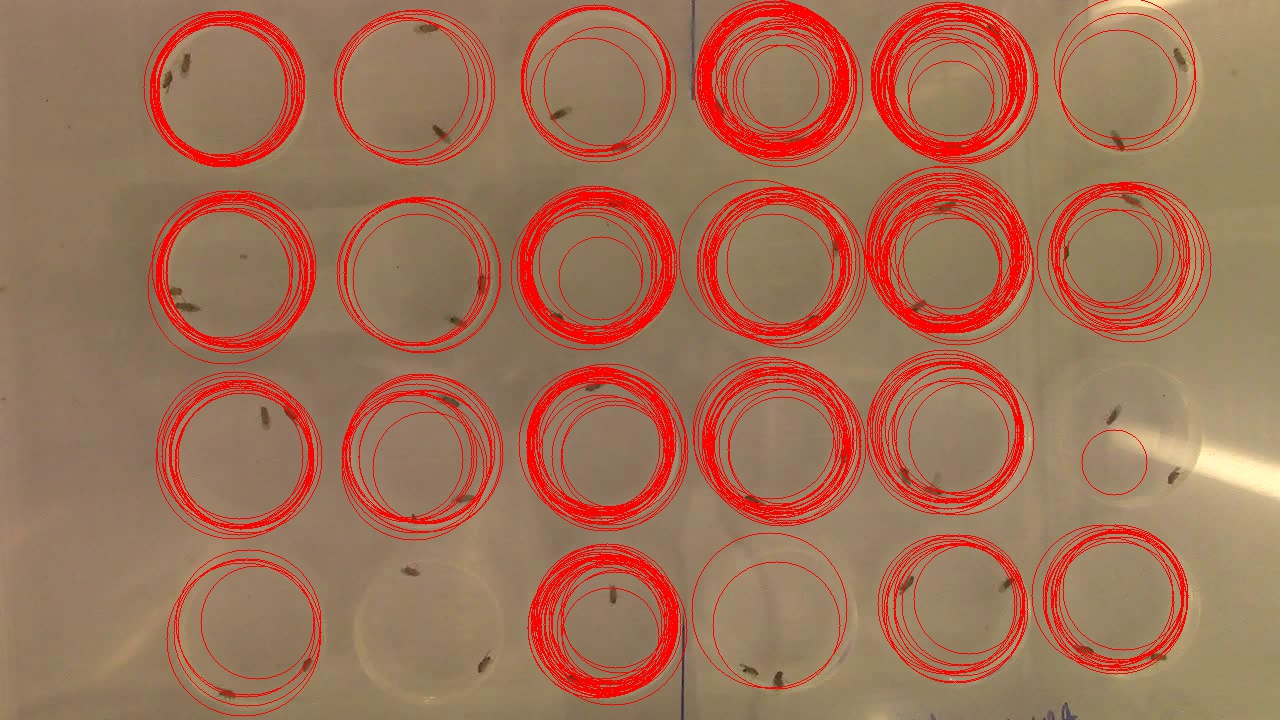
\includegraphics[width=0.8\textwidth]{simple_hough_circle}
\caption{Hough圆检测的结果}
\label{fig:simple_hough_circle}
\end{figure}

对Hough圆检测得到的圆进行聚类,得到如图~\ref{fig:containers_adaptive}所示的结果。图~\ref{fig:containers_adaptive}中显示的是\ref{sec:container_split}章中活动台提取算法的结果。参数$param_1$和$param_2$经过13次自适应后,最终取值为$param_1=param_2=56.5$,每个活动台周围平均检测到$3\sim 4$个Hough圆。从图~\ref{fig:containers_adaptive}可以看出,聚类后基本可以准确地找到活动台的位置,但是因为部分活动台周围仅能找到较少数目的Hough圆,且位置的准确性也存在较大的误差,因而检测结果与实际位置偏差较大。图~\ref{fig:containers_adaptive}中仅显示了检测结果不太准确的情况,在个别极端情况下,果蝇活动台提取算法还有可能出现漏检、重复检测的情况,即部分活动台被检出了2次,而有的活动台则一次都没有被检测到。通过选择足够多的视频帧、选取合适的聚类中心可以减少上述问题发生的概率,与此同时也会增加算法的计算量。

\begin{figure}[htb]
\centering
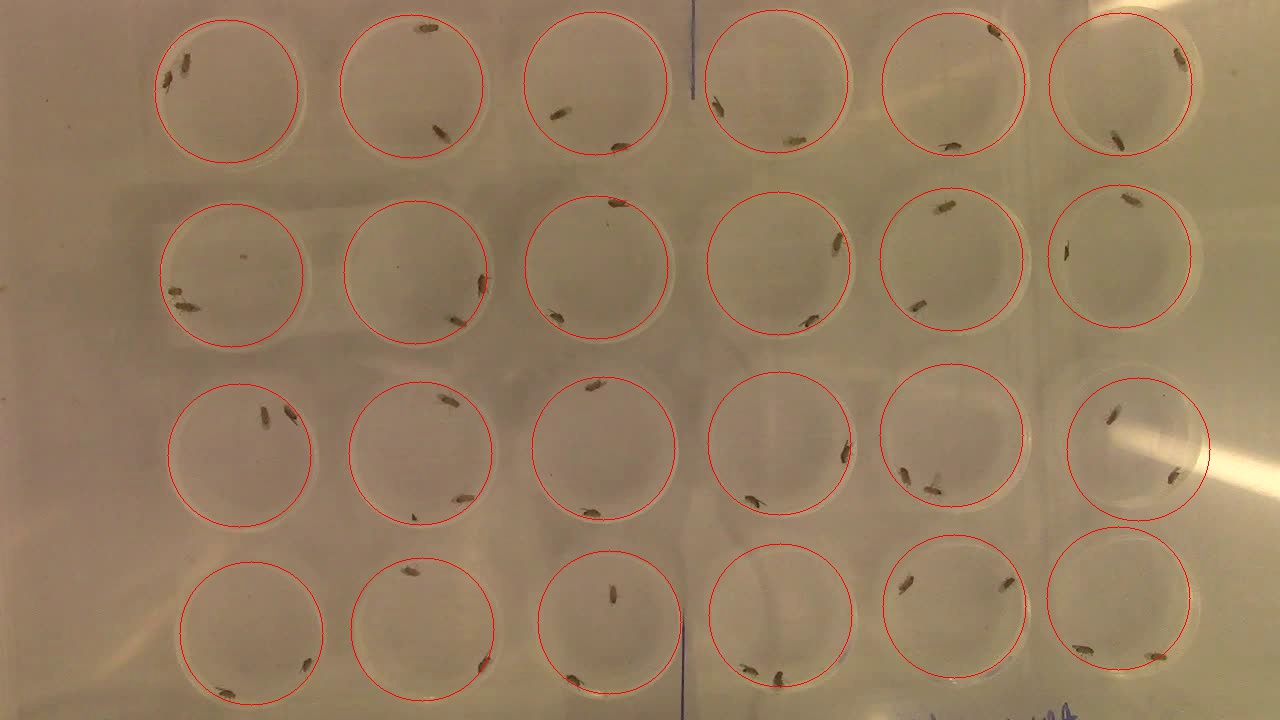
\includegraphics[width=0.8\textwidth]{containers_adaptive}
\caption{自适应的果蝇活动台检测结果}
\label{fig:containers_adaptive}
\end{figure}

最后,对图~\ref{fig:containers_adaptive}中的结果进一步采用基于固定排列的活动台提取算法,得到图~\ref{fig:containers_fixed_array}所示的结果。图~\ref{fig:containers_fixed_array}中果蝇活动台的位置和大小均比较准确。

\begin{figure}[htb]
\centering
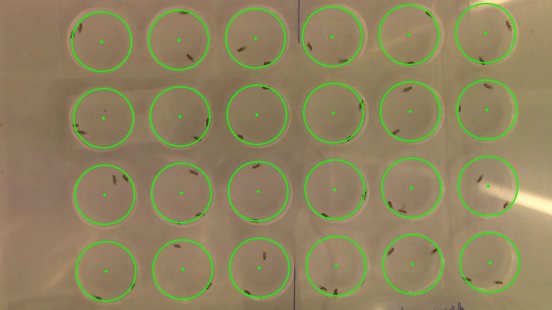
\includegraphics[width=0.8\textwidth]{containers_fixed_array}
\caption{基于特定排列的果蝇活动台检测结果}
\label{fig:containers_fixed_array}
\end{figure}

\section{小结}

本章主要介绍了果蝇活动台提取模块。首先介绍了基于形状检测算法的果蝇活动台提取算法,通过Hough圆检测参数的自适应,使得算法能较好的适应不同的视频。其次,基于特定排列模式的果蝇行为视频,通过对果蝇活动台位置进行建模,建立图像坐标系和理想坐标系之间的仿射变换,完成果蝇活动台位置的进一步优化。通过利用果蝇活动台的位置信息,提高了检测的准确性,提升了系统的可用性。最终完成果蝇活动台的切割,为接下来的果蝇轮廓提取做准备工作。


% \chapter{果蝇轮廓提取和追踪} \label{chapter:fly_contour}

果蝇轮廓提取的目标是从果蝇视频中分离出果蝇活动台、果蝇身体和果蝇翅膀,进而为提取果蝇特征做准备。其中,果蝇活动台一般为纯色背景,在不同的拍摄环境下,可能存在程度不等的噪声;果蝇身体一般为深色,和浅色的果蝇活动台差异明显,相对来说比较容易区分;果蝇翅膀呈半透明状,在视频中,果蝇翅膀区域的灰度往往介于身体和活动台之间,且翅膀的姿态往往存在较多的变化,如,果蝇可能存在振单翅、振双翅、收拢翅膀等,在不同的姿态下翅膀也表现出不同的形态。果蝇的翅膀是果蝇行为的重要特征,其中,果蝇在打架时振翅可能是一种威胁信号;而在求偶行为中,振翅也是求偶的信号。准确提取出果蝇翅膀是果蝇行为分析的基本要求。

此外,果蝇视频的拍摄环境不统一,给果蝇的身体轮廓提取带来很大的考验。现有的果蝇轮廓提取算法一般对果蝇的拍摄环境有专门的限制,比如,特定的光照条件、较高精度的拍摄设备等,给果蝇行为分析算法增加了不少限制。

本章提出一种基于背景模型的果蝇轮廓提取算法,在单高斯背景模型的基础上,对视频进行初步建模,进而在初步模型的基础上,分离果蝇活动台、果蝇身体和果蝇翅膀,通过对活动台单独建模,得到更准确的果蝇活动台模型。

\section{果蝇轮廓提取的背景模型}

果蝇身体轮廓提取的目标是从包含单独果蝇活动台的视频中,分离出多只果蝇的身体、翅膀和活动台的背景。和一般的前景物体提取不同,果蝇活动台相对比较简单,受到运动、光照等因素的影响较小;前景部分果蝇的面积和背景相比较小;前景目标在整个视频中始终存在;此外,果蝇翅膀的特殊性也对背景模型提出很高的精度要求。

%%%%%%%%%%%%%%%%%%%%%%%%%%%%%%%%%%%%%%%%%%%%%%%%%%%%%%%%%%%%
%                      果蝇活动台的初步模型
%%%%%%%%%%%%%%%%%%%%%%%%%%%%%%%%%%%%%%%%%%%%%%%%%%%%%%%%%%%%
\subsection{果蝇视频的初步背景建模}\label{sec:fly_bg_model_basic}

本章介绍一种算法,通过用单高斯背景模型和亮度畸变模型对果蝇视频进行背景建模,实现对果蝇身体和翅膀轮廓的提取。

首先,从果蝇视频中抽取$K$帧$I_{1}, I_{2}, \ldots, I_{K}$,并计算该$K$帧视频的均值$\mu$和方差$\sigma^2$,作为活动台的均值和方差;

然后,计算视频帧$I_{1}, I_{2}, \ldots, I_{K}$的亮度畸变。亮度畸变的计算公式如(\ref{eq:brightness_distortion})所示\cite{shadow_2000}:
\begin{equation}\label{eq:brightness_distortion}
\alpha(m,n) = \frac{
        \frac{I_R(m, n)\mu_R(m, n)}{\sigma_R^2(m, n)} +
        \frac{I_G(m, n)\mu_G(m, n)}{\sigma_G^2(m, n)} +
        \frac{I_B(m, n)\mu_B(m, n)}{\sigma_B^2(m, n)}
    }{
        \left[\frac{\mu_R(m, n)}{\sigma_R(m, n)}\right]^2 +
        \left[\frac{\mu_G(m, n)}{\sigma_G(m, n)}\right]^2 +
        \left[\frac{\mu_B(m, n)}{\sigma_B(m, n)}\right]^2
    },
\end{equation}
其中,$m, n$表示图像中元素的坐标,R、G、B表示色彩通道。亮度畸变可以较好的描述图像中的阴影部分,而果蝇的翅膀呈现的半透明状态和阴影在一定程度上类似。亮度畸变的引入有助于提取果蝇翅膀\cite{chexiangqian}。视频的亮度畸变$\alpha$描述了视频帧和平均值,即活动台背景$\mu$的偏离程度,其中,果蝇身体所在区域和活动台背景差异较大,亮度畸变的取值一般来说也比较小;果蝇翅膀次之,果蝇活动台部分一般最高。通过对亮度畸变进行阈值化可以大致分离出果蝇的身体、翅膀和果蝇活动台。

进一步计算视频亮度畸变的空间分布,计算$I_{1}, I_{2}, \ldots, I_{K}$的亮度畸变$\alpha_1, \alpha_2, \ldots, \alpha_{K}$的均方差,即$\textrm{RMS}(\alpha)$,并利用$\textrm{RMS}(\alpha)$对亮度畸变$\alpha$进行归一化。$\textrm{RMS}(\alpha)$的表达式如下所示:
\begin{equation} \label{eq:alpha_RMS}
\textrm{RMS}\left(\alpha(m,n)\right) =
\sqrt{\frac{\sum_{i=1}^{K} \left(\alpha_{i}(m,n)-\bar{\alpha}(m,n)\right)^2}{K}},
\end{equation}
其中,$\bar{\alpha}$表示$K$视频的亮度畸变$\alpha_1, \alpha_2, \ldots, \alpha_K$的均值,根据式(\ref{eq:brightness_distortion})的定义,易得$\bar{\alpha} = 1$。用$\textrm{RMS}(\alpha)$对$\alpha$进行归一化的原因在于,受限于拍摄条件,果蝇视频中一般存在噪声,且在视频的不同区域噪声的幅度不尽相同。

$\textrm{RMS}(\alpha)$的取值主要由两部分构成:一部分是果蝇身体和翅膀的运动,另一部分是视频拍摄过程中带来的噪声。当果蝇频繁移动时,$\textrm{RMS}(\alpha)$的取值主要由前一部分构成。使用$\textrm{RMS}(\alpha)$对$\alpha_i$进行归一化,可以降低将噪声误判为果蝇身体的可能。

归一化后的亮度畸变$\hat{\alpha}(m,n) = \alpha(m,n)/\textrm{RMS}\left(\alpha(m,n)\right)$。进一步将$\hat{\alpha}$归一化到区间$[0, 1]$,得到最终亮度畸变$\tilde{\alpha}$。果蝇的身体和翅膀可以通过对$\tilde{\alpha}$的阈值化来实现:
\begin{flalign} \label{eq:body_and_wing_model_basic}
I_{i, body} &= \left(\tilde{\alpha}_i < \tau_{body}\right), \\
I_{i, wing} &= \left(\tilde{\alpha}_i > \tau_{body} \quad \text{and} \quad \tilde{\alpha}_i < \tau_{wing}\right),
\end{flalign}
其中,$\tau_{body}$和$\tau_{wing}$通过经验设定。经验表明,$\tau_{body}$和$\tau_{wing}$对实验环境不敏感,在不同的拍摄场景和实验环境下波动很小。

此外,$\textrm{RMS}(\alpha)$还反应了果蝇的活动情况,果蝇移动频繁的区域,$\textrm{RMS}(\alpha)$较大,果蝇移动不频繁的区域,$\textrm{RMS}(\alpha)$取值较小。通过$\textrm{RMS}(\alpha)$可以得到精确果蝇活动台内径\cite{chexiangqian}。对$\textrm{RMS}(\alpha)$做阈值化处理:
\begin{equation}
I_{active} = \left( \textrm{RMS}(\alpha) > \tau_{active} \right),
\end{equation}
其中$\tau_{active}$取$\textrm{RMS}(\alpha)$的平均值即可。$I_{active}$表示了果蝇活动区域,求$I_{active}$的最小外包圆,得到果蝇活动台的精确位置。上述实现的前提是果蝇在活动台中频繁移动,且移动轨迹覆盖果蝇活动台的最外侧,上述条件很容易满足:经验表明,果蝇喜欢沿活动台的边缘追逐、爬行,利用果蝇的活动求解果蝇活动台的算法在大多数情况下都试用。

综上,果蝇活动台的均值$\mu$、方差$\sigma^2$和亮度畸变的均方差$\textrm{RMS}(\alpha)$构成了果蝇活动台轮廓提取的初步模型,记该模型为$\textrm{M}_1$。

综上,果蝇背景模型$\textrm{M}_1$的训练步骤参见算法~\ref{alg:fly_contour_model1_train}。

\begin{algorithm}
\caption{基于背景模型$\textrm{M}_1$的果蝇轮廓提取算法(训练)}
\label{alg:fly_contour_model1_train}
\begin{algorithmic}[1]
\INPUT
    \Statex 果蝇行为视频;
\OUTPUT
    \Statex 果蝇活动台背景的均值$\mu$;
    \Statex 果蝇活动台背景的方差$\sigma^{2}$;
    \Statex 果蝇活动台背景亮度畸变的均方差$\textrm{RMS}(\alpha)$;

\State 对果蝇视频进行$K$帧抽样,得到视频帧$I_{1}, I_{2}, \ldots, I_{K}$;
\State 计算视频帧$I_{1}, I_{2}, \ldots, I_{K}$的均值$\mu$和方差$\sigma^2$;
\For {$i = 1 \text{ to } K$;}
    \State 根据式(\ref{eq:brightness_distortion})计算视频帧$I_{i}$的亮度畸变$\alpha_i$;
\EndFor
\State 根据果蝇视频的亮度畸变$\alpha_1, \alpha_2, \ldots, \alpha_K$,求解亮度畸变的均方差$\textrm{RMS}(\alpha)$;
\State 输出果蝇活动台背景的均值$\mu$、果蝇活动台背景的方差$\sigma^{2}$和果蝇活动台背景亮度畸变的均方差$\textrm{RMS};(\alpha)$
\end{algorithmic}
\end{algorithm}

根据果蝇背景模型$\textrm{M}_1$进行果蝇身体轮廓提取的流程如算法~\ref{alg:fly_contour_model1_test}所示。

\begin{algorithm}
\caption{基于背景模型$\textrm{M}_1$的果蝇轮廓提取算法}
\label{alg:fly_contour_model1_test}
\begin{algorithmic}[1]
\INPUT
    \Statex 果蝇视频帧$I$;
    \Statex 果蝇活动台背景的均值$\mu$;
    \Statex 果蝇活动台背景的方差$\sigma^{2}$;
    \Statex 果蝇活动台背景亮度畸变的均方差$\textrm{RMS}(\alpha)$;
    \Statex 果蝇身体和翅膀阈值$\tau_{body}$和$\tau_{wing}$;
\OUTPUT
    \Statex 果蝇身体$I_{body}$和果蝇翅膀$I_{wing}$;

\State 根据式(\ref{eq:brightness_distortion})计算视频帧$I$的亮度畸变$\alpha$;
\State 根据式(\ref{eq:alpha_RMS})计算果蝇视频的正则化的亮度畸变$\hat{\alpha}$;
\State 将$\hat{\alpha}$归一化到区间$[0, 1]$,得到$\tilde{\alpha}$;
\State 根据$\tau_{body}$和$\tau_{wing}$对果蝇视频进行阈值化,得到果蝇身体$I_{body}$和翅膀$I_{wing}$;
\State 输出果蝇身体$I_{body}$和果蝇翅膀$I_{wing}$。
\end{algorithmic}
\end{algorithm}

背景模型$\textrm{M}_1$中,根据式(\ref{eq:body_and_wing_model_basic}) 可以得到果蝇的身体和翅膀。但是,在上面的做法中存在一个问题:我们假设$\mu$和$\sigma^2$分别表示果蝇背景的均值和方差,实际上$\mu$和$\sigma^2$表示的是果蝇视频的均值和方差,$\mu$和$\sigma^2$的计算中没有消除果蝇身体和果蝇翅膀对果蝇活动台的影响,因而存在一定的误差。下面对可能带来的误差做简单分析。

假设视频中共有2只果蝇,且2只果蝇的身体尺寸大小相同\footnote{一般来说,雌性果蝇的身体比雄性稍大。},面积均为$S_{fly}$;在整个视频时间段,果蝇投影面积不变;果蝇活动台的面积为$S_{c}$。按照背景模型$\textrm{M}_1$,果蝇的身体和翅膀被算入果蝇活动台背景,当果蝇身体和翅膀均匀的出现在果蝇活动台中时,背景模型中果蝇身体和翅膀所占的比例为:
\begin{equation}\label{eq:fly_area_ratio}
r = \frac{2S_{fly}}{S_{c}}.
\end{equation}

式(\ref{eq:fly_area_ratio})大致刻画了背景模型$\textrm{M}_1$中存在系统误差的量级。一般来说,果蝇面积相对活动台的面积很小,模型的误差也较小。但实际上,果蝇均匀的出现在容器内的假设不成立。一般来说,果蝇的活动范围往往局限于很小的区间,如活动台侧壁。在果蝇活动频繁的区域,$\textrm{M}_1$模型的果蝇活动台亮度明显偏暗。在亮度畸变的计算公式(\ref{eq:brightness_distortion})中,$I$和$\mu$是等价的,偏暗的背景和偏暗的果蝇都会使得亮度畸变值偏低,进而体现在式(\ref{eq:body_and_wing_model_basic})中,影响果蝇轮廓提取的准确性。为此,我们在本章节接下来的内容中提出一种更精确的果蝇轮廓提取模型。

%%%%%%%%%%%%%%%%%%%%%%%%%%%%%%%%%%%%%%%%%%%%%%%%%%%%%%%%%%%%
%                      果蝇活动台的精确模型
%%%%%%%%%%%%%%%%%%%%%%%%%%%%%%%%%%%%%%%%%%%%%%%%%%%%%%%%%%%%
\subsection{果蝇活动台的精确建模}\label{sec:fly_bg_model_model2}

背景模型$\textrm{M}_1$的问题主要在果蝇身体和翅膀被记入了果蝇活动台背景部分,为了解决该问题,可以首先分离果蝇活动台和果蝇身体、果蝇翅膀,具体方法用式(\ref{eq:body_and_wing_model_basic}),然后单独对果蝇活动台部分建立背景模型。下面具体介绍该算法的实现步骤。

首先,对视频帧$I_{1}, I_{2}, \ldots, I_{K}$建立单高斯背景模型模型$\textrm{M}_1$。根据式(\ref{eq:body_and_wing_model_basic})分割果蝇身体$I_{body, i}$、翅膀$I_{wing, i}$和活动台,并计算果蝇活动台的均值$\mu'$和方差$\sigma'^2$:
\begin{flalign}\label{eq:gaussian_model2}
\mu'(m, n) &= \frac{\sum_{i=1}^{K}F_i(m, n)I_i(m, n)}{\sum_{i=1}^{K}F_i(m, n)} \\
\sigma^{\prime 2}(m, n) &=
    \frac
        {\sum_{i=1}^{K}F_i(m, n)\left(I_i(m, n) - \mu'(m,n)\right)^{2}}
        {\sum_{i=1}^{K}F_i(m, n)}
\end{flalign}
其中,$F_i(m,n)$取0或1,$F_i(m,n) = 0$表示帧$I_i$在坐标$(m, n)$的像素对应果蝇身体或翅膀,$F_i(m,n) = 1$表示对应像素属于果蝇活动台。$\textrm{M}_1$模型提取的果蝇身体和翅膀并不完全准确,但对式(\ref{eq:gaussian_model2})来说,我们仅希望$\textrm{M}_1$不要将果蝇身体或翅膀判定为果蝇活动台,反之并没有严格的要求。所以在本步骤中,可以适当对式(\ref{eq:body_and_wing_model_basic})中的$\tau_{body}$和$\tau_{wing}$加以调整,使果蝇的身体和翅膀条件更加宽松。

同样的,计算视频的亮度畸变公式更新为:
\begin{equation}\label{eq:brightness_distortion_model2}
\alpha'_{m,n} = \frac{
        \frac{I_R(m, n)\mu^{\prime}_R(m, n)}{\sigma_R^{\prime 2}(m, n)} +
        \frac{I_G(m, n)\mu^{\prime}_G(m, n)}{\sigma_G^{\prime 2}(m, n)} +
        \frac{I_B(m, n)\mu^{\prime}_B(m, n)}{\sigma_B^{\prime 2}(m, n)}
    }{
        \left[\frac{\mu^{\prime}_R(m, n)}{\sigma^{\prime}_R(m, n)}\right]^2 +
        \left[\frac{\mu^{\prime}_G(m, n)}{\sigma^{\prime}_G(m, n)}\right]^2 +
        \left[\frac{\mu^{\prime}_B(m, n)}{\sigma^{\prime}_B(m, n)}\right]^2
    }.
\end{equation}

亮度畸变$\alpha_1, \alpha_2, \ldots, \alpha_K$的均方差$\textrm{RMS}(\alpha')$的计算公式为:
\begin{equation}
\textrm{RMS}\left(\alpha'(m, n)\right) = \sqrt{
    \frac{
        \sum_{i=1}^{K}F_i(m,n)\left(\alpha'_{i}(m, n)-\bar{\alpha'}(m, n)\right)^2}
        {\sum_{i=1}^{K}F_i(m,n)}
}.
\end{equation}

果蝇活动台的均值$\mu'$和方差$\sigma'^2$和亮度畸变的均方差$\textrm{RMS}(\alpha')$构成新的精确模型,记为$\textrm{M}_2$。利用$\textrm{M}_2$计算果蝇的身体和翅膀的流程和第\ref{sec:fly_bg_model_basic}章的过程类似,首先,利用$\textrm{RMS}(\alpha')$对亮度畸变$\alpha'$的归一化:
\begin{equation}
\hat{\alpha}'(m, n) = \frac{\alpha'(m, n)}{\textrm{RMS}\left(\alpha'(m, n)\right)},
\end{equation}

进而将$\hat{\alpha}'$归一化到区间$[0, 1]$,得到$\tilde{\alpha}'$。通过阈值化$\tilde{\alpha}'$,完成果蝇身体和翅膀的轮廓提取。对视频帧$I_i$,果蝇身体$I_{i, body}$和果蝇翅膀$I_{i,wing}$的计算表达式为:
\begin{flalign}\label{eq:fly_contour_model2}
I_{i, body} &= \left(\tilde{\alpha}'_i < \tau_{body}\right), \\
I_{i, wing} &= \left(\tilde{\alpha}'_i > \tau_{body} \quad \text{and} \quad \tilde{\alpha}'_i < \tau_{wing}\right).
\end{flalign}

因为剔除了果蝇身体和翅膀对背景的影响,因而式(\ref{eq:fly_contour_model2})中得到的果蝇身体$I_{i, body}$和果蝇翅膀$I_{i,wing}$更加精确。

背景模型$\textrm{M}_2$的完整求解流程可以用算法~\ref{alg:fly_contour_model2_train}来描述:

\begin{algorithm}
\caption{果蝇精确}
\label{alg:fly_contour_model2_train}
\begin{algorithmic}[1]
\INPUT
    \Statex 果蝇行为视频;
    \Statex 果蝇活动台背景模型$\textrm{M}_1$;
\OUTPUT
    \Statex 果蝇活动台均值$\mu'$;
    \Statex 果蝇活动台方差$\sigma^{\prime 2}$;
    \Statex 果蝇活动台亮度畸变的均方差$\textrm{RMS}(\alpha')$;
\State 对果蝇视频进行$K$帧采样,得到视频帧$I_{1}, I_{2}, \ldots, I_{K}$;
\For {$i = 1 \text{ to } K$; }
    \State 利用$\textrm{M}_1$模型,计算视频帧$I_i$中的果蝇身体$I_{i, body}$和翅膀$I_{i, wing}$;
\EndFor
\State 根据式(\ref{eq:gaussian_model2}),计算更新的果蝇活动台均值$\mu'$和方差$\sigma^{\prime 2}$
\For {$i = 1 \text{ to } K$; }
    \State 求视频帧$I_{i}$的亮度畸变$\alpha'_{i}$;
\EndFor
\State 计算果蝇行为视频中活动台的亮度畸变$\alpha'_{1}, \alpha'_{2}, \ldots, \alpha'_{K}$的均方差$\textrm{RMS}(\alpha')$;
\State 输出果蝇活动台均值$\mu'$、果蝇活动台方差$\sigma^{\prime 2}$、果蝇活动台亮度畸变的均方差$\textrm{RMS}(\alpha')$。
\end{algorithmic}
\end{algorithm}

根据背景模型$\textrm{M}_2$求果蝇身体和翅膀的流程和算法~\ref{alg:fly_contour_model1_test}类似,在此不做详细的介绍。

\subsection{果蝇身体轮廓的自适应}

最后,本章简要介绍使用果蝇的身体尺寸对果蝇身体进行自适应的算法。作为对模型$\textrm{M}_2$的必要补充,自适应的引入可以提高算法的鲁棒性。

首先,对视频进行$K$帧抽样,并使用第\ref{sec:fly_locate}章中果蝇身体尺寸求解算法,计算每一帧$I_i$中果蝇身体的尺寸$(a_i, b_i)$。然后,求解果蝇身体尺寸$(a_1, b_1),(a_2, b_2), \ldots, (a_K, b_K)$的中位数,得到果蝇身体的最终尺寸$(a, b)$。需要注意的是,为了得到更加准确的果蝇身体尺寸,应该仅计算果蝇连通域数目和果蝇数目相等的帧。

在假设果蝇身体为椭圆形的情况下,计算果蝇身体约等于$S=\pi ab$。根据背景模型$\textrm{M}_2$,得到果蝇身体部位$I_{body}$和翅膀部位$I_{wing}$,分别求身体部位的实际面积$S_{body}$和翅膀部位的实际面积$S_{wing}$,并分别引入变量$r_{body}$和$r_{wing}$:
\begin{flalign}\label{eq:fly_contour_ratio_adptive}
r_{body} &= \frac{S_{body}}{2S}, \\
r_{wing} &= \frac{S_{wing}}{2S}.
\end{flalign}

对于视频中包含果蝇数目不为2的情况,需要对(\ref{eq:fly_contour_ratio_adptive})进行相应的调整。

分别对果蝇翅膀和果蝇身体进行自适应,流程如下:如果$r_{wing} < r_{wing,lower}$,说明翅膀的面积偏小,应该增加$\tau_{wing}$的值以增加检测到的果蝇翅膀面积。反之,如果$r_{wing} > r_{wing, upper}$,则说明果蝇的翅膀面积偏大, 应该减小$\tau_{wing}$以降低检测到的果蝇翅膀的面积。$\tau_{wing}$的调整可以采用增加或者减少一个固定的值$\Delta_{wing}$来实现,即$\tau^{\{i+1\}}_{wing} = \tau^{\{i\}}_{wing} \pm \Delta_{wing}$,其中$i$表示自适应的次数,$\tau^{\{i\}}_{wing}$表示第$i$轮自适应的翅膀阈值参数。根据调整后的翅膀阈值$\tau^{\{i+1\}}_{wing}$重新计算果蝇翅膀$I_{wing}$和对应的面积$S_{wing}$,进而重新计算$r_{wing}$。对上述步骤进行若干次,即可实现翅膀的自适应。

对果蝇身体部位的自适应过程与之类似。在果蝇翅膀自适应完成后,进行果蝇身体的自适应。当$r_{body} < r_{body, lower}$时,说明果蝇身体的面积偏小,需要减小$\tau_{body}$来增加检测到的果蝇身体的面积;反之,如果$r_{body} > r_{body, upper}$,说明果蝇身体的面积偏大,需要增加$\tau_{body}$的值。对上述步骤进行若干次调整,即可完成身体部分的自适应。

果蝇身体和翅膀的自适应算法进一步提高了果蝇轮廓提取算法的鲁棒性,使得算法对不同拍摄环境下的果蝇行为视频都能取得较好的结果。

%%%%%%%%%%%%%%%%%%%%%%%%%%%%%%%%%%%%%%%%%%%%%%%%%%%%%%%%%%%%
%                      果蝇的定位和追踪
%%%%%%%%%%%%%%%%%%%%%%%%%%%%%%%%%%%%%%%%%%%%%%%%%%%%%%%%%%%%
\section{果蝇的定位和追踪} \label{sec:fly_discrimination_and_track}

\subsection{果蝇身体的定位}\label{sec:fly_locate}

得到果蝇的身体和翅膀的区域后,需要进一步的计算每只果蝇的位置。令$I_{fly}$表示果蝇身体和翅膀所在区域,求$I_{fly}$的连通域。当果蝇活动台中有2只果蝇时,理论上应该出现2个连通区域,且每个连通区域和单只果蝇分别对应。但实际上,考虑到果蝇行为视频中,果蝇在部分情况下存在身体接触、甚至求偶时果蝇完全抱在一起,使得$I_{fly}$中仅存在一个连通区域;在部分情况下,果蝇侧立在活动台的侧壁,果蝇翅膀遮盖住果蝇部分身体,比如果蝇腹部,使得果蝇腹部的灰度明显比正常的果蝇身体亮,在根据式(\ref{eq:body_and_wing_model_basic})求解果蝇身体时出现果蝇身体在腹部出现明显的断裂,导致$I_{fly}$中的连通区域数目超过果蝇的数目。此外,果蝇视频中可能存在光线的亮度、噪声等都可能对连通域的数目带来影响,造成连通域数目和果蝇数目不一致的问题。

在果蝇连通域数目$k$和果蝇数目$K$一致时,我们可以认为每个连通域和果蝇身体相对应。果蝇的身体轮廓可以被建模成椭圆\cite{chexiangqian}。但是,求解连通域的最小外包椭圆相对比较困难,我们可以用最小外包矩形代替。最小外包矩形可以用参数$\{(x, y), (A, B), \theta\}$来表示,其中$(x, y)$表示外包矩形中心的坐标,$(A, B)$表示外包矩形的长和宽,$\theta$表示外包矩形长边的方向。在椭圆形假设下,果蝇身体的长轴和短轴分别为$(a, b) = (A/2, B/2)$。求解最小外包矩形的计算复杂度为线性复杂度,不超过最小外包矩形的面积\cite{Freeman:1975:DME:360881.360919}。通过求解最小外包矩形的参数,可以得到果蝇身体的位置、大小和方向。

对于连通域数目和果蝇身体数目不一致的情况,应分两种情况:连通域的数目$k$大于果蝇数目$K$;或连通域的数目$k$小于果蝇数目$K$。下面分别对上述情况加以考虑。

$k>K$时,一般是因为果蝇的身体某部分可能出现了不连通的情况,可以通过对果蝇身体$I_{fly}$的坐标进行聚类,将身体所在像素的坐标聚类为果蝇的数目,聚类结果的每一类别对应一只果蝇。和上述求解果蝇身体位置、大小的方式一样,通过求解最小外包矩形求解果蝇身体参数$\{(x, y), (A, B), \theta\}$。根据问题的特点,选择使用采用Single-Linkage的层次聚类(Hierarchical Clustering)算法\cite{rokach2005clustering},像素点的距离采用4-近邻距离。

$k<K$时,使用细胞分割算法${}^{\cite{cell_seg_2010}}$。连通域数目小于果蝇数目时,一般是因为果蝇之间存在身体接触。细胞分割算法专门用于分离接触的目标,当物体有小面积接触时效果较好,在大面积重合时算法的性能不尽人意,主要是因为细胞分割算法只能把重叠区域分配给其中1个物体,因而有重叠的目标都比实际要小。该算法的主要思路也是对坐标进行聚类,但是在聚类时考虑到了每个像素的权重不同,位于连通域边缘的像素具有较小的权重,而位于连通域中心的像素具有较大的权重。聚类一般采用混合高斯模型实现,距离尺度使用欧氏距离。通过\cite{cell_seg_2010}中的算法,将果蝇身体划分成不同的连通域,并通过求解最小外包矩形求解果蝇身体的参数$\{(x, y), (A, B), \theta\}$。上述算法在处理求偶时完全重叠的果蝇时会出现问题,在今后的研究中可以综合考虑果蝇的姿态等,以减少上述算法对果蝇身体分割带来的影响。

通过上述步骤,求出分离的果蝇,并求出每只果蝇的基本身体参数$\{(x, y), (A, B), \theta\}$。

\subsection{果蝇的追踪}\label{sec:fly_track}

根据第\ref{sec:fly_locate}章中的算法,可以确定每一帧中果蝇身体的位置$(x, y)$和身体朝向$\theta$。但是,在不同的帧间,我们需要确定不同果蝇的对应关系,即编号问题。此外,根据果蝇轮廓的外包矩形只能判断身体的朝向,并不能直接确定果蝇头部的方向,还需要进一步判断果蝇头部的朝向。

首先,考虑果蝇之间的对应关系。果蝇的身体结构比较简单,不同个体之间的差异性不大,在实验环境下,很难通过视频的图形学特征判断果蝇的编号。为此,可以根据运动信息来判定:
% \DeclareMathOperator*{\argmin}{arg\,min}
\begin{equation}\label{eq:fly_dicrimination}
\underset{n_{1},n_2, \ldots, n_K}{arg\,min}
\sum_{i=1}^K\|\vec{P}_{c, n_i} - \vec{P}_{c, i}\|_2^2
\end{equation}

其中,$\vec{P}_{c, i}$表示第$i$只果蝇身体重心的位置,$n_i$表示下一帧中果蝇$i$的新编号,$n_i$的取值是$\left\{1,2,\ldots,K\right\}$的一个排列组合。通过最小化式(\ref{eq:fly_dicrimination})中的目标函数,基本可以保证果蝇序号不发生交换。

外包矩形给出了果蝇身体的参数$\left\{(x, y), (a, b), \theta\right\}$,其中$\theta$只给出了果蝇身体的朝向,果蝇的头部方向可能是$\theta$或$\theta+\pi$。为了确定果蝇头部的方向,可以考虑以下几种特征:
\begin{enumerate}
\item 根据果蝇的形态特征进行判断;
\item 根据果蝇的运动特征进行判断;
\item 根据果蝇上一帧的结果进行判断;
\end{enumerate}

首先,根据果蝇的形态特征进行判断。考虑到果蝇的身体形态特征,从图形学的角度判断果蝇的头部和尾部的方法不太多,目前比较常用的是根据头部和尾部的灰度差异判断。果蝇的翅膀一般收缩在尾部,因而尾部的亮度会比头部稍微高一些。图像亮度较低的是头部,图像亮度较高的是尾部。此外,还有根据果蝇头部和尾部轮廓的曲率判断果蝇头部和尾部的方式。

其次,根据果蝇在帧间的运动特征进行判断。正常情况下,果蝇会选择向前移动。计算每两帧之间果蝇的运动方向,其头部朝向在大多数情况下和果蝇的运动方向应该是一致的,尾部朝向和运动方向相反。但是考虑到果蝇在部分情况下可能会静止,或者存在较小的后退,比如,在打架行为中,果蝇为了蓄力往往会有一个后挫动作。通过运动方向来判断果蝇的头部和尾部存在一定的问题。

最后,可以根据果蝇的上一帧结果进行判断。参考式(\ref{eq:fly_dicrimination})中的方案,通过最小化果蝇头部和尾部在帧间移动距离的平方和,完成果蝇头部和尾部的识别。对于第$i$帧中果蝇$k$,首先,求出该果蝇可能的头部位置和尾部位置$\vec{P}_{0}$和$\vec{P}_{1}$,
\begin{equation}\label{eq:fly_head_tail_dist}
\underset{i_0, i_1}{arg\,min} \left\|\vec{P}_{i_0} - \vec{P}_{h}\right\|_2^2 + \left\|\vec{P}_{i_1} - \vec{P}_{t}\right\|_2^2.
\end{equation}
其中,$\vec{P}_{h}$和$\vec{P}_{t}$分别表示第$i-1$帧中果蝇$k$的头部和尾部的位置,$i_0$、$i_1$是$\left\{0, 1\right\}$的一个排列组合。通过最小化头部和尾部的移动距离的平方和,保证果蝇头部和尾部移动的连续性,基本可以保证在正常移动情况下果蝇头部和尾部在视频中的一致性。

最后,本章综合采用果蝇的移动方向和上一阵果蝇的位置进行果蝇头部和尾部的判断。如果果蝇在前后帧的移动距离大于某阈值时,利用果蝇的移动方向确定果蝇的头部和尾部;否则,利用上一帧的果蝇头部和尾部的位置信息确定当前帧下果蝇的头部和尾部。


%%%%%%%%%%%%%%%%%%%%%%%%%%%%%%%%%%%%%%%%%%%%%%%%%%%%%%%%%%%%
%                      果蝇轮廓提取的结果和分析
%%%%%%%%%%%%%%%%%%%%%%%%%%%%%%%%%%%%%%%%%%%%%%%%%%%%%%%%%%%%
\section{果蝇轮廓提取的结果和分析}\label{sec:chap4_experiments}

本文对不同环境下拍摄的果蝇视频进行果蝇身体检测和追踪。如图~\ref{fig:bg_model_origin}所示,来自4组不同拍摄环境下的视频,从左到右依次记为视频(a)、(b)、(c)、(d),每段视频长度约为10分钟,视频的大小约为200$\times$200,清晰度和分辨率各不相同,亮度上也存在较大的差异。此外,视频中还存在相当的噪声,从视频帧(a)中可以看出,果蝇活动台的中心有浅黄色的果蝇食物,活动台的侧壁存在明暗不同的反光。在视频(b)、(c)和(d)中也存在程度不同的上述情况。除视频拍摄环境、视频质量外,(a)、(b)、(c)、(d)视频中包含不同的果蝇尺度和姿态,图~\ref{fig:bg_model_origin}中包括了果蝇侧立、正趴、追尾以及求偶等不同的形态,在不同的形态中,果蝇的翅膀也呈现出不同的形态特征,如,(a)中翅膀收在尾部,(b)中右下角的果蝇翅膀展开,(c)、(d)中果蝇翅膀因侧立等原因呈现出细、尖的特点。

针对上述不同视频,分别用大律法、背景模型$\textrm{M}_1$和背景模型$\textrm{M}_2$进行果蝇轮廓的提取。其中,背景模型$\textrm{M}_1$和背景模型$\textrm{M}_1$的参数阈值$\tau_{wing} = 0.63, \tau_{body} = 0.42$,并对阈值$\tau_{wing}$和$\tau_{body}$进行自适应,自适应的步长为0.01,最多自适应步数10次。

\begin{figure}
\centering
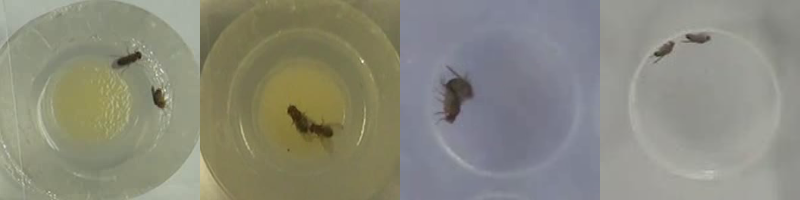
\includegraphics[width=0.9\textwidth]{bg_model_origin}
\caption{果蝇视频示例}
\label{fig:bg_model_origin}
\end{figure}

大律法提取果蝇轮廓的结果如图~\ref{fig:bg_model_ostu}所示,其中,白色、黑色分别表示果蝇身体和活动台背景。图~\ref{fig:bg_model_ostu}表明,大律法提取果蝇轮廓的结果很差,视频(a)、(d)中果蝇轮廓和活动台背景混杂在一起,无法分开。这是因为视频(a)、(d)的拍摄环境比较简单,果蝇活动台的颜色并不均一,其暗色部分和果蝇翅膀效果比较接近,仅仅依靠像素灰度无法有效的提取果蝇的身体和翅膀。

\begin{figure}
\centering
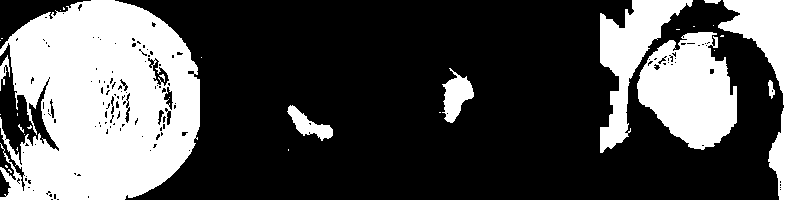
\includegraphics[width=0.9\textwidth]{bg_model_ostu}
\caption{大律法求果蝇轮廓结果}
\label{fig:bg_model_ostu}
\end{figure}

下面详细讨论背景模型$\textrm{M}_1$和背景模型$\textrm{M}_2$。以视频(d)为例,计算视频模型中的背景图像,并计算和原始的视频帧的差,其中视频图像如图~\ref{fig:frame}所示,模型$\textrm{M}_1$和$\textrm{M}_2$求解的活动台背景如图~\ref{fig:frame_mean_model1}和图~\ref{fig:frame_mean_model2}所示。

\begin{figure}
\centering
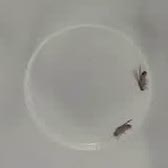
\includegraphics[width=0.25\textwidth]{frame}
\caption{原始果蝇视频}\label{fig:frame}
\end{figure}

\begin{figure}
\centering
\subcaptionbox{模型$\textrm{M}_1$的背景\label{fig:frame_mean}} {
    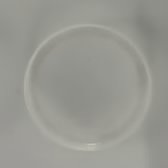
\includegraphics[width=0.25\textwidth]{frame_mean}
}
\hspace{10pt}
\subcaptionbox{背景与视频帧的差\label{fig:frame_delta}} {
    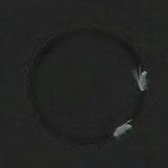
\includegraphics[width=0.25\textwidth]{frame_delta}
}
\caption{背景模型$\textrm{M}_1$的果蝇活动台模型}
\label{fig:frame_mean_model1}
\end{figure}

\begin{figure}
\centering
\subcaptionbox{模型$\textrm{M}_2$的背景\label{fig:bg_mean}} {
    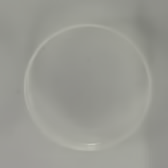
\includegraphics[width=0.25\textwidth]{bg_mean}
}
\hspace{10pt}
\subcaptionbox{背景与视频帧的差\label{fig:bg_delta}} {
    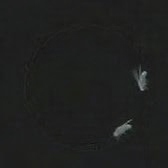
\includegraphics[width=0.25\textwidth]{bg_delta}
}
\caption{背景模型$\textrm{M}_2$下的果蝇活动台模型}
\label{fig:frame_mean_model2}
\end{figure}

图~\ref{fig:frame_mean_model1}和图~\ref{fig:frame_mean_model2}中,左侧是对应背景模型求得的活动台背景,右侧是活动台背景和原始果蝇视频帧的差。考虑到活动台背景和原始果蝇视频帧的差值中存在负值,在图~\ref{fig:frame_mean_model1}和图~\ref{fig:frame_mean_model2}中对像素值加上某个常量,使之最小值为0。对比图~\ref{fig:frame_mean_model1}和图~\ref{fig:frame_mean_model2}的背景,背景模型$\textrm{M}_1$求得的活动台在边缘区域明显比背景模型$\textrm{M}_2$要暗,这是一个因为果蝇习惯沿果蝇互动台侧壁移动。对比差值更能清楚的反映出该问题,在~\ref{fig:frame_delta}的边缘明显存在偏暗的圈,而在~\ref{fig:bg_delta}中,除果蝇身体所在区域外,其余区域基本为黑色,即果蝇活动台的背景部分被很好的剔除掉。

下面看视频帧的亮度畸变。同样对图~\ref{fig:frame}中的图像,分别用背景模型$\textrm{M}_1$和背景模型$\textrm{M}_2$求亮度畸变,结果如图~\ref{fig:model_alpha}所示。视频的亮度畸变的取值一般在$[0, 2]$之间,为了便于表示,我们把亮度畸变归一化到区间$[0, 255]$。在图~\ref{fig:model_alpha}中,果蝇身体所在的区域最暗,其次是果蝇翅膀,最后是果蝇活动台。只需要对亮度畸变进行阈值化即可得到最终的果蝇身体和果蝇翅膀。对比~\ref{fig:frame_alpha}和~\ref{fig:bg_alpha},很容易看出背景模型$\textrm{M}_2$比背景模型$\textrm{M}_1$的改进。在~\ref{fig:bg_alpha}中,果蝇活动台区域的取值更加一致,且和果蝇身体、翅膀的取值相差较大,因而采用阈值化可以得到更准确的果蝇身体和翅膀。

\begin{figure}
\centering
\subcaptionbox{模型$\textrm{M}_1$下的亮度畸变$\alpha$\label{fig:frame_alpha}} {
    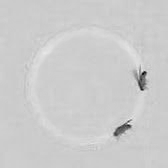
\includegraphics[width=0.25\textwidth]{frame_alpha}
}
\hspace{10pt}
\subcaptionbox{模型$\textrm{M}_2$下的亮度畸变$\alpha'$\label{fig:bg_alpha}} {
    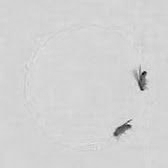
\includegraphics[width=0.25\textwidth]{bg_alpha}
}
\caption{背景模型的亮度畸变}
\label{fig:model_alpha}
\end{figure}

利用背景模型$\textrm{M}_1$和背景模型$\textrm{M}_2$提取果蝇轮廓的结果参见图~\ref{fig:bg_model_result_1}、 图~\ref{fig:bg_model_result_2}。图中,黑色、白色、灰色分别表示果蝇活动台、果蝇身体和果蝇翅膀。图~\ref{fig:bg_model_result_2}中,对于来自4个视频的帧,本文提出的背景模型都能准确的提取出果蝇的轮廓,比如,视频(b)中正趴在容器底部的果蝇张开的翅膀,以及视频(d)中趴在容器壁上侧立的果蝇的翅膀尖,均有良好的表现。同样的,图~\ref{fig:bg_model_result_1}也能找到视频中的果蝇身体和翅膀,但与此同时,该模型也会将大量的果蝇活动台判定为果蝇翅膀。这也说明对活动台单独建模的必要性。

\begin{figure}[htb]
\centering
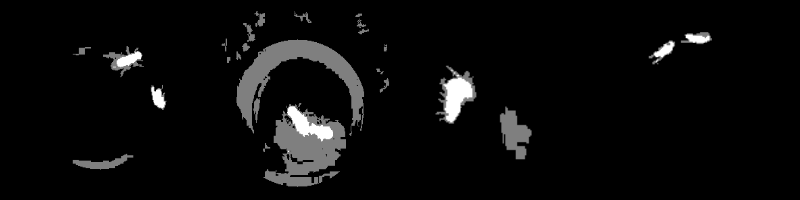
\includegraphics[width=0.9\textwidth]{bg_model_result_1}
\caption{背景模型$\textrm{M}_1$求果蝇轮廓结果}
\label{fig:bg_model_result_1}
\end{figure}

\begin{figure}[thb]
\centering
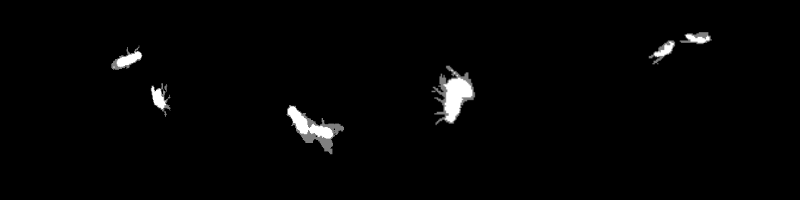
\includegraphics[width=0.9\textwidth]{bg_model_result_2}
\caption{背景模型$\textrm{M}_2$求果蝇轮廓结果}
\label{fig:bg_model_result_2}
\end{figure}

\section{小结}
针对果蝇轮廓提取的问题,本章提出了一种基于背景模型的算法。该算法先通过对果蝇视频进行初步建模,大致分割出果蝇的身体、翅膀和活动台后,进一步对活动台单独建模,得到更加准确的背景模型,进而实现果蝇身体轮廓的准确提取。仿真结果表明,本文提出的算法可以适应不同拍摄环境,具有较好的鲁棒性。



% \chapter{果蝇行为识别实验}\label{chap:fly_behavior_detection}

果蝇行为一般包括打架行为、求偶行为等,不同的行为有不同的特点。本章通过实验,在第\ref{chapter:fly_contour}章中果蝇轮廓提取算法的基础上,使用车向前提出的果蝇特征提取算法和果蝇行为识别算法\cite{chexiangqian},完成整个果蝇打架行为的检测。实验结果表明,计算机可以比人工更好的处理果蝇行为分析视频。

%%%%%%%%%%%%%%%%%%%%%%%%%%%%%%%%%%%%%%%%%%%%%%%%%%%%
%                   果蝇行为视频的数据标定
%%%%%%%%%%%%%%%%%%%%%%%%%%%%%%%%%%%%%%%%%%%%%%%%%%%%
\section{果蝇行为视频的数据标定} \label{sec:fly_behavior_character}

一般来说,果蝇行为学中关注的果蝇行为主要包括果蝇的打架行为、求偶行为等\cite{copulation_2009}。果蝇的打架行为和果蝇的求偶行为存在不同的外在特点,在进行果蝇行为识别中一般也采用不同的果蝇特征。本实验主要针对果蝇的打架行为进行检测。

实验所用的果蝇行为视频主要来自北京大学饶毅实验室,果蝇行为经过相关专家标定,具有较高的可信性和一致性。

%%%%%%%%%%%%%%%%%%%%%%%%%%%%%%%%%%%%%%%%%%%%%%%%%%%%
%                   果蝇行为视频的数据标定
%%%%%%%%%%%%%%%%%%%%%%%%%%%%%%%%%%%%%%%%%%%%%%%%%%%%
\section{果蝇行为识别的流程}

果蝇行为识别的步骤一般分为:果蝇活动台提取和分割、果蝇轮廓提取和追踪、果蝇特征提取、果蝇行为识别几个步骤。如图~\ref{fig:fly_detection_procedure}所示。

\begin{figure}
\centering
\begin{tikzpicture}
\node [block, text width=10em] (split_chambers) {\heiti 果蝇活动台分割};
\node [block, text width=10em, below = 0.5cm of split_chambers] (extract_contour) {\heiti 果蝇身体轮廓提取};
\node [block, text width=10em, below = 0.5cm of extract_contour] (feature_extract) {\heiti 果蝇特征提取};
\node [block, text width=10em, below = 0.5cm of feature_extract] (behavior_detect) {\heiti 果蝇行为分析};

\path [arrow] (split_chambers) -- (extract_contour);
\path [arrow] (extract_contour) -- (feature_extract);
\path [arrow] (feature_extract) -- (behavior_detect);
\end{tikzpicture}
\caption{果蝇行为识别自动化分析流程}
\label{fig:fly_detection_procedure}
\end{figure}

其中,第\ref{chapter:container_split}章介绍了果蝇活动台分割算法,介绍了如何从包含多个果蝇活动台的视频中切分出包含单个果蝇活动台的视频,在果蝇活动台排列存在一定规律时,还可以利用基于特定排列的果蝇活动台分割算法进行活动台分割。

根据第\ref{chapter:fly_contour}章介绍的果蝇轮廓提取算法,提取果蝇的身体轮廓。对某一个视频进行背景建模后,得到的模型对视频中的每一帧进行处理,得到视频帧中的果蝇身体和翅膀轮廓。求果蝇身体和翅膀区域的连通域,将其中面积太小的判定为噪声并删除,然后将连通区域划分成分离的果蝇。对分离的果蝇进行编号,并跟踪果蝇的运动情况,判定果蝇的头部和尾部。在此基础上,计算果蝇的特征。

果蝇的特征提取分为3步\cite{chexiangqian}:
\begin{enumerate}
\item 果蝇特征点的初步定位;
\item 果蝇特征点的SDM算法迭代更新;
\item 根据果蝇特征点进行果蝇姿态的重构。
\end{enumerate}

计算果蝇的特征点需要对果蝇进行椭球形建模,提取果蝇身体周围的8个特征点:果蝇的头部$\vec{p}_{h}$、尾部$\vec{p}_{t}$、左侧$\vec{p}_{l}$、右侧$\vec{p}_{r}$、背部$\vec{p}_{top}$、腹部$\vec{p}_{bottom}$、左翅膀根部$\vec{p}_{l,wing}$、右翅膀根部$\vec{p}_{r,wing}$。上述8个特征点中,果蝇的头部、尾部、左侧、右侧、背部、腹部主要根据果蝇身体连通域的外包矩形计算得到,果蝇的左翅膀根部和右翅膀根部通过翅膀轮廓处理得到,一般来说,翅膀表现出较尖、细的特征,在视频中不容易直接找到,可以分按照以下步骤进行:首先,找到果蝇翅膀和果蝇身体的连接处$\vec{p}_{lwing,root}$和$\vec{p}_{rwing,root}$;其次,计算翅膀的张开角度,对果蝇翅膀上的每一个像素点计算其相对翅膀根部的角度,并进行直方图统计,直方图中取值最大的角度就对应了果蝇翅膀的角度;最后,根据果蝇翅膀的长度和翅膀张开的角度,计算果蝇翅膀根据的位置$\vec{p}_{l,wing}$和$\vec{p}_{r,wing}$。

计算完成果蝇特征点后,采用SDM算法进行特征点的迭代更新,得到更准确的果蝇特征点。SDM算法最开始被用于人脸识别中人脸特征点的定位,车向前将SDM算法应用于果蝇特征点的迭代更新文章\cite{chexiangqian},取得了较好的效果。本文也采用该论文介绍的子空间SDM算法,对提取到的果蝇特征点位置进行更新。最后,使用子空间的SDM算法迭代更新后的果蝇特征点对果蝇的身体姿态进行重建,得到更精确的果蝇姿态,如果蝇翅膀倾角等。

最后,根据果蝇的姿态等特征,计算果蝇打架行为的特征。果蝇的打架行为包括直视、后挫、前冲等3个步骤,既包含了帧内果蝇之间的空间关系,还包含了时间上复杂的逻辑关系,因而果蝇打架行为的特征也包括了帧内特征和帧间特征\cite{chexiangqian}。对打架行为特征,经过数据标定,共得到10个视频、400个果蝇打架行为样本,对上述样本上训练SVM分类器,得到针对果蝇打架行为的分类器。

需要注意的是,上述果蝇特征点提取、利用SDM算法对果蝇特征点进行迭代更新、果蝇姿态重构、果蝇打架特征的计算等算法参照车向前论文\cite{chexiangqian}。

\section{果蝇行为识别结果}

经过训练和测试,在果蝇打架数据集上,使用5-fold交叉校验,果蝇打架行为分类器取得了的$84.3\%$准确率和$76.5\%$的召回率。

\section{小结}

经过试验,我们得到了完整的果蝇行为识别系统,该系统可以得到优于人工的标定结果。


% \chapter{果蝇行为识别服务网站的系统设计}

果蝇识别学是动物行为学中的重要组成部分,而自动化的分析果蝇行为对果蝇行为学的研究有重要意义。虽然不同实验室的果蝇研究环境不尽相同,但是果蝇的身体特征相对比较简单、个体之间的差异性并不明显,因而给统一的分析方法提供了可能。在解决了果蝇环境的差异对果蝇行为识别带来的困难后,可以考虑将果蝇行为识别系统推广至其他果蝇拍摄环境。为此,本文专门开发了一个基于果蝇行为识别的网站,通过在网站上提交果蝇视频,并下载识别的结果,实现自动化的果蝇行为识别。果蝇行为识别网站服务方面,主要工作包括两部分:果蝇行为识别程序和网站建设。

\section{果蝇行为识别程序}

果蝇行为识别程序的主要目标在于,通过自动化的果蝇行为分析算法,分析输入的果蝇行为视频,并将分析的结果输出。果蝇行为识别程序希望提供尽可能方便的接口,和灵活可变的配置参数,以便其他程序的调用。下面将介绍果蝇行为识别程序的模块和开发环境。

\subsection{果蝇行为识别的模块结构}

果蝇行为自动化分析主要分为几个模块:活动台的分割、果蝇身体的提取和追踪、果蝇特征的提取、果蝇行为识别。对应到程序中,果蝇行为识别程序主要划分为如图~\ref{fig:fly_detection_procedure2}所示的几个模块,各模块的功能分别如下:
\begin{description}
\item[活动台的分割] 输入包含多个果蝇活动台的视频,输出多个包含单独果蝇活动台的视频,以及对应活动台视频的相关信息,包括:果蝇活动台的中心、果蝇活动台的大小、果蝇活动台移入视频的时间、果蝇活动台移出视频的时间;其中,模块可以输出csv格式的文件,用来保存切分视频的结果;
\item[果蝇身体的提取和追踪] 输入包含单个果蝇活动台的视频,输出果蝇活动台在整个视频中的位置和大小、果蝇身体的尺寸、视频中每一帧果蝇身体和翅膀的区域、每只果蝇身体的轮廓;其中,模型将果蝇的背景模型保存成文件,以方便以后使用;
\item[果蝇特征的提取] 输入果蝇行为视频和果蝇身体提取和追踪模块的结果,输出每一帧中每只果蝇特征点的位置,以及根据果蝇特征点计算得到的果蝇姿态;此外,该模块还可以输出果蝇的速度、加速度等运动信息,并将全部的特征保存到文件;
\item[果蝇行为识别] 输入每只果蝇的位置信息、姿态信息,输出果蝇在整个时间段的行为分析结果。此外,模块还可以输出果蝇行为的特征。
\end{description}

\begin{figure}
\centering
\begin{tikzpicture}
\node [block, text width=10em] (split_chambers) {\heiti 果蝇活动台分割};
\node [block, text width=10em, below = 0.5cm of split_chambers] (extract_contour) {\heiti 果蝇身体轮廓提取};
\node [block, text width=10em, below = 0.5cm of extract_contour] (feature_extract) {\heiti 果蝇特征提取};
\node [block, text width=10em, below = 0.5cm of feature_extract] (behavior_detect) {\heiti 果蝇行为分析};

\path [arrow] (split_chambers) -- (extract_contour);
\path [arrow] (extract_contour) -- (feature_extract);
\path [arrow] (feature_extract) -- (behavior_detect);
\end{tikzpicture}
\caption{果蝇行为识别自动化分析流程}
\label{fig:fly_detection_procedure2}
\end{figure}

\subsection{果蝇行为识别程序的开发和编译环境}

果蝇行为识别程序主要部署在Linux操作系统下,其开发环境的主要依赖关系包括:
\begin{itemize}
\item OpenCV 2.4.x
\item CMake >= 3.0
\end{itemize}

OpenCV被广泛的应用在果蝇行为识别程序中\cite{itseez2015opencv,itseez2014theopencv}。OpenCV的全称Open Source Computer Vision Library,是一个免费、开源的计算机视觉方面的库,该库以BSD开源软件协议发布,提供了大量的计算机图形学中的基本操作接口,如视频、图像的IO操作、基础的图形学操作如色域转换、高级的图像特征算法如方向梯度直方图(Histogram of oriented gradient,HOG)算法\cite{dalal2005histograms}、尺度不变特征变换(Scale-invariant feature transform,SIFT)算法\cite{lowe1999object}等,以及部分计算机学习库,如SVM等。此外,OpenCV还兼容不同的平台,可以方便的部署到Windows、Linux等系统上。本文使用了稳定版本的OpenCV 2.4.x,主要利用OpenCV库提供的图形学操作进行图形的基本处理,以及机器学习库进行测试等。

对于果蝇行为识别程序而言,果蝇行为视频的处理大概能做到接近实时,即程序运行的时和果蝇视频的长度在同一个量级。和其他果蝇行为分析系统相比,该程序的运行速度并不算慢\cite{dankert2009automated},但是仍然存在较大的发展空间。对于一个摄像头,一般会同时拍摄超过20个果蝇活动台,这就给程序处理带来较大的压力。为此,在维持现有算法基本不变的情况下,可以从OpenCV库的选择入手。目前,OpenCV的最新稳定版本为 2.4.13,但是最新的开发版本已经到了 3.2.0。最新的3.2.0版本除了提供更开放的计算机图形学算法外,还为大部分的计算机图形学操作、矩阵运算等提供了GPU运算接口,对于大量的计算机图形学操作,可以大大提高程序运行的效率。

在程序的编译方面,使用CMake作为程序的make工具,并使用gcc编译器,对果蝇行为识别程序。编译完成后,得到可执行程序DetectFly,通过命令行参数指定输入的视频、果蝇行为视频的类型(打架、求偶)、输出结果的文件名等。可执行程序通过分析果蝇视频,将果蝇的行为输出到特定的文件中。外部程序可以通过调用可执行程序,得到果蝇行为视频中果蝇的所有行为。

\section{果蝇行为识别网站}

在果蝇行为自动分析程序DetectFly的基础上,本文搭建了果蝇行为自动分析的网站,对外提供果蝇行为识别服务。果蝇行为识别网站提供了用户注册、用户登录、果蝇行为识别任务的添加、果蝇行为识别任务结果下载等功能。下面简单介绍果蝇行为识别的自动化分析网站。

\subsection{网站的功能介绍}

果蝇行为识别网站的链接:\url{http://gu.ee.tsinghua.edu.cn/drosophila}。目前,网站主要包含以下功能:用户的注册、用户登录、果蝇行为视频任务的创建、果蝇行为视频上传、果蝇行为视频分析结果下载等模块。

果蝇行为识别网站存在用户管理功能。果蝇行为识别需要大量的计算资源,因而对用户的使用需要一定的条件,以便进行资格审查。首先,需要用户进行注册,只有注册用户才能使用网站提供的果蝇行为识别功能。网站的注册页面如图~\ref{fig:website_register}所示,用户需要提供包括姓名、研究机构、电子邮箱等基本信息,以便进一步联系。

\begin{figure}
\centering
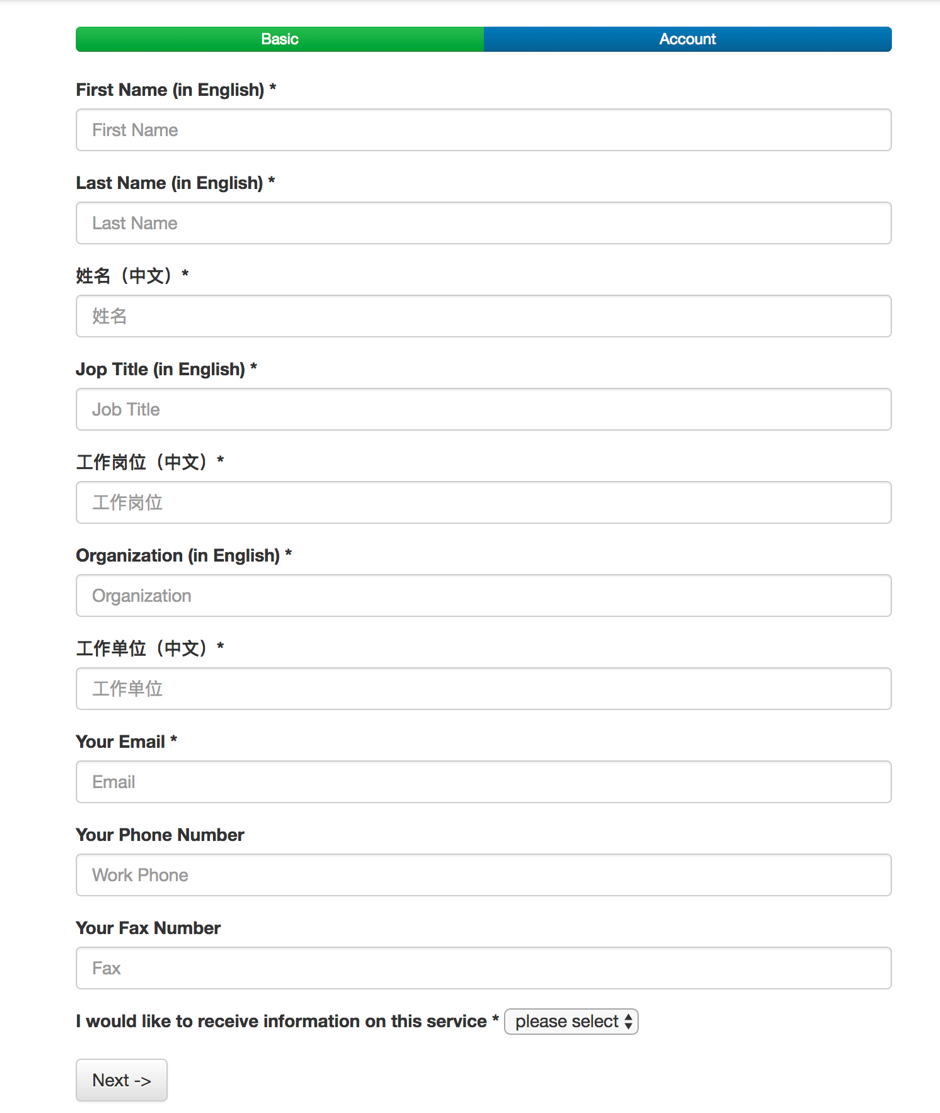
\includegraphics[width=0.8\textwidth]{website_register}
\caption{果蝇行为识别网站的注册}
\label{fig:website_register}
\end{figure}

在用户提交注册申请后,网站后台会给管理员发送邮件,等待管理员确认用户资格后,用户可以正常登陆和使用网站提供的果蝇行为识别服务。网站的登录页面如图~\ref{fig:website_login}所示。

\begin{figure}
\centering
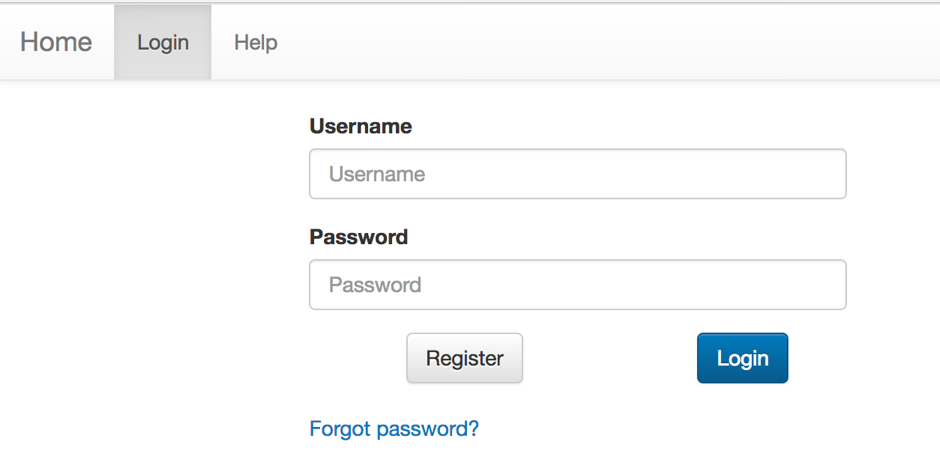
\includegraphics[width=0.8\textwidth]{website_login}
\caption{果蝇行为识别网站的登录}
\label{fig:website_login}
\end{figure}

完成登录后,可以创建果蝇行为识别任务,并上传果蝇行为视频。图~\ref{fig:website_new_mission}界面显示了创建果蝇行为识别任务的界面,目前,网站支持2种果蝇行为识别任务:打架行为和求偶行为。创建任务时,需要选定果蝇行为识别的任务类型、创建的任务名称,还支持对任务进行简单的评注,以便日后查找。对于已经完成的任务,还提供了不同的过滤列表,以便用户查询。过滤列表有以下4种:
\begin{itemize}
\item All - 全部任务列表
\item Failed - 失败的任务列表
\item Succeeded - 成功的任务列表
\item Incomplete - 未完成任务列表
\end{itemize}

\begin{figure}
\centering
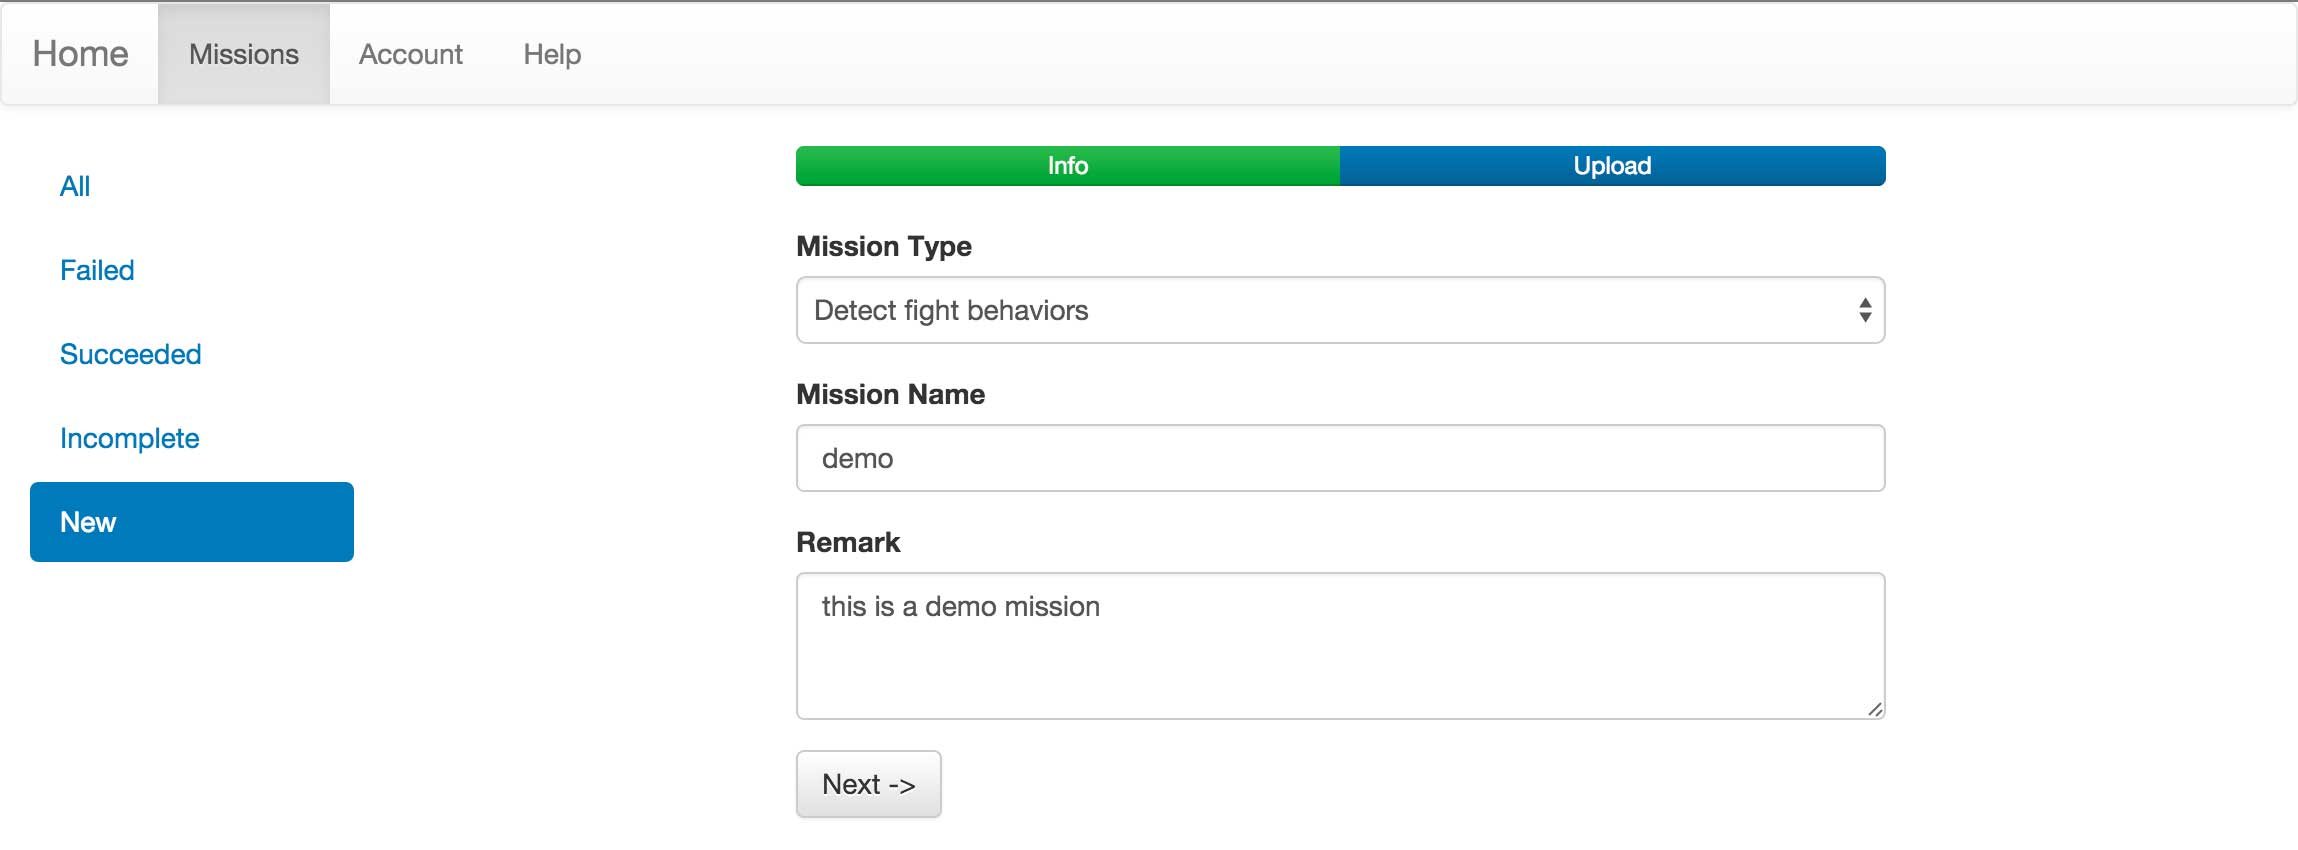
\includegraphics[width=0.8\textwidth]{website_new_mission}
\caption{创建果蝇行为识别任务}
\label{fig:website_new_mission}
\end{figure}

在完成任务创建后,需要上传果蝇行为视频。果蝇行为视频文件的大小较大,此步骤需要花费一定时间。一般来说,错误的果蝇活动台分割会给后续的果蝇行为识别任务带来难以预计的结果,这会给网站带来大量无用的计算,并消耗用户大量的时间。在综合考虑后,网站要求用户自行进行果蝇活动台的分割任务,同时要求上传的果蝇行为视频为包含一个单独的果蝇活动台的果蝇行为视频。如图~\ref{fig:website_new_mission}所示,视频文件上传完成后,点击"submit"即可提交果蝇分析任务。任务状态[Mission State]会有如下几种:
\begin{itemize}
\item Pending – 任务正在等待被处理
\item Processing – 任务正在处理中(这一步是计算过程,需要等待较长时间)
\item Succeeded – 任务处理完成
\item Failed – 任务处理失败
\end{itemize}

\begin{figure}
\centering
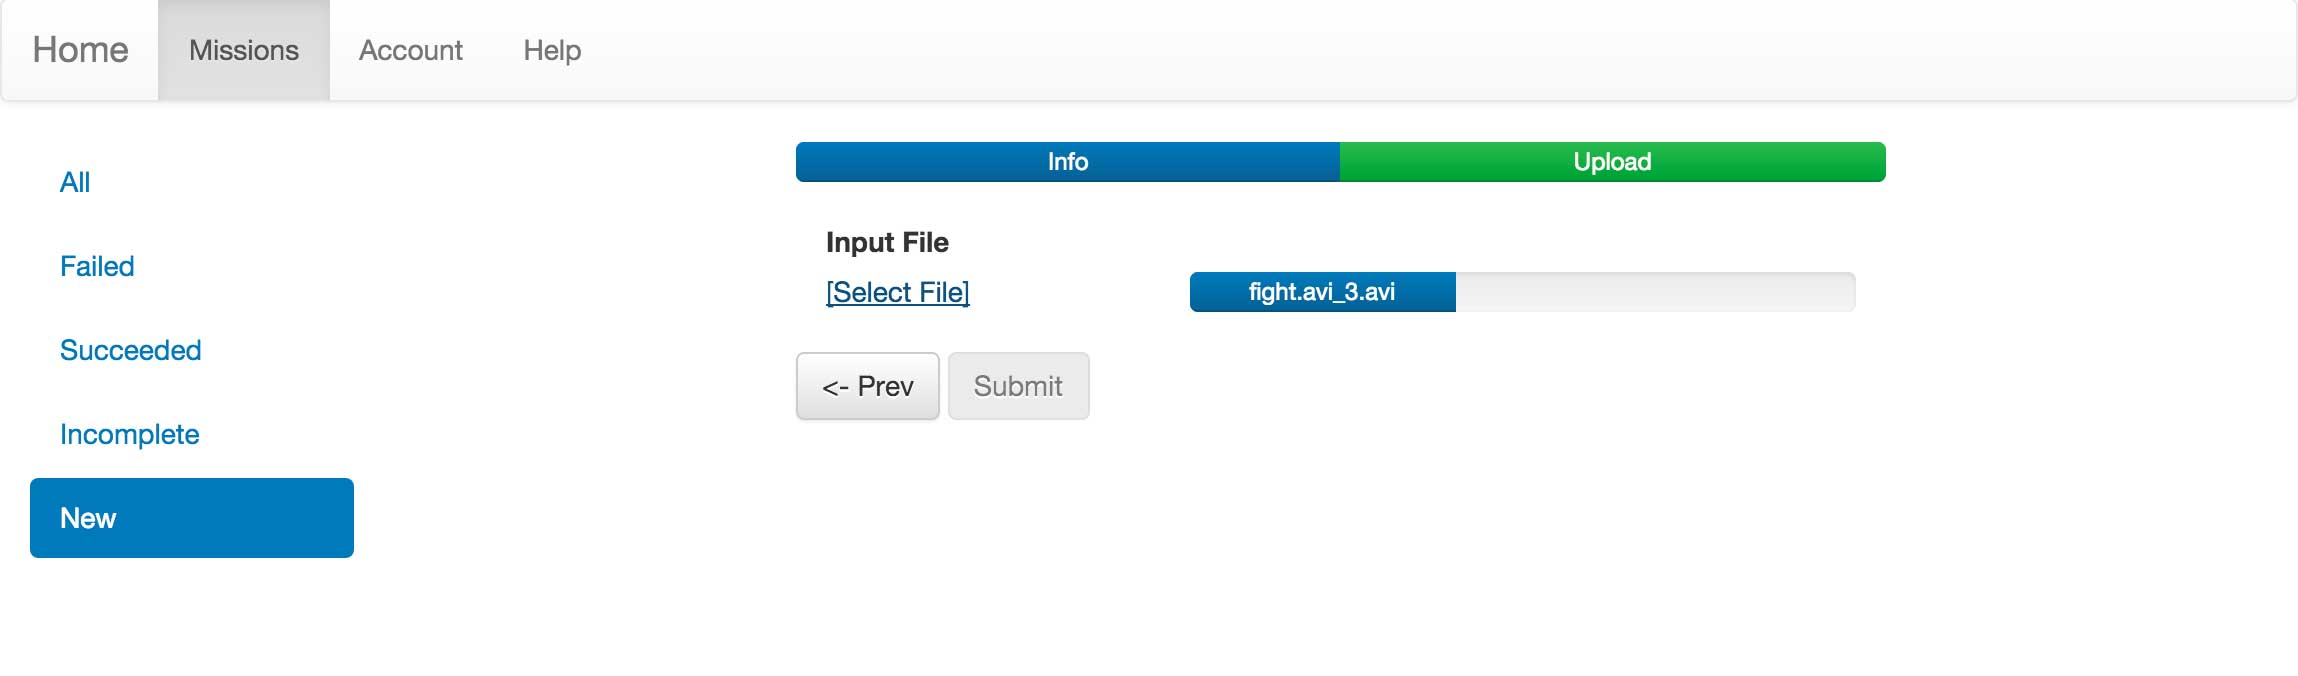
\includegraphics[width=0.8\textwidth]{website_upload_video}
\caption{上传果蝇行为视频}
\label{fig:website_upload_video}
\end{figure}

在此阶段,用户看到如图~\ref{fig:website_waiting_for_result}界面。

\begin{figure}
\centering
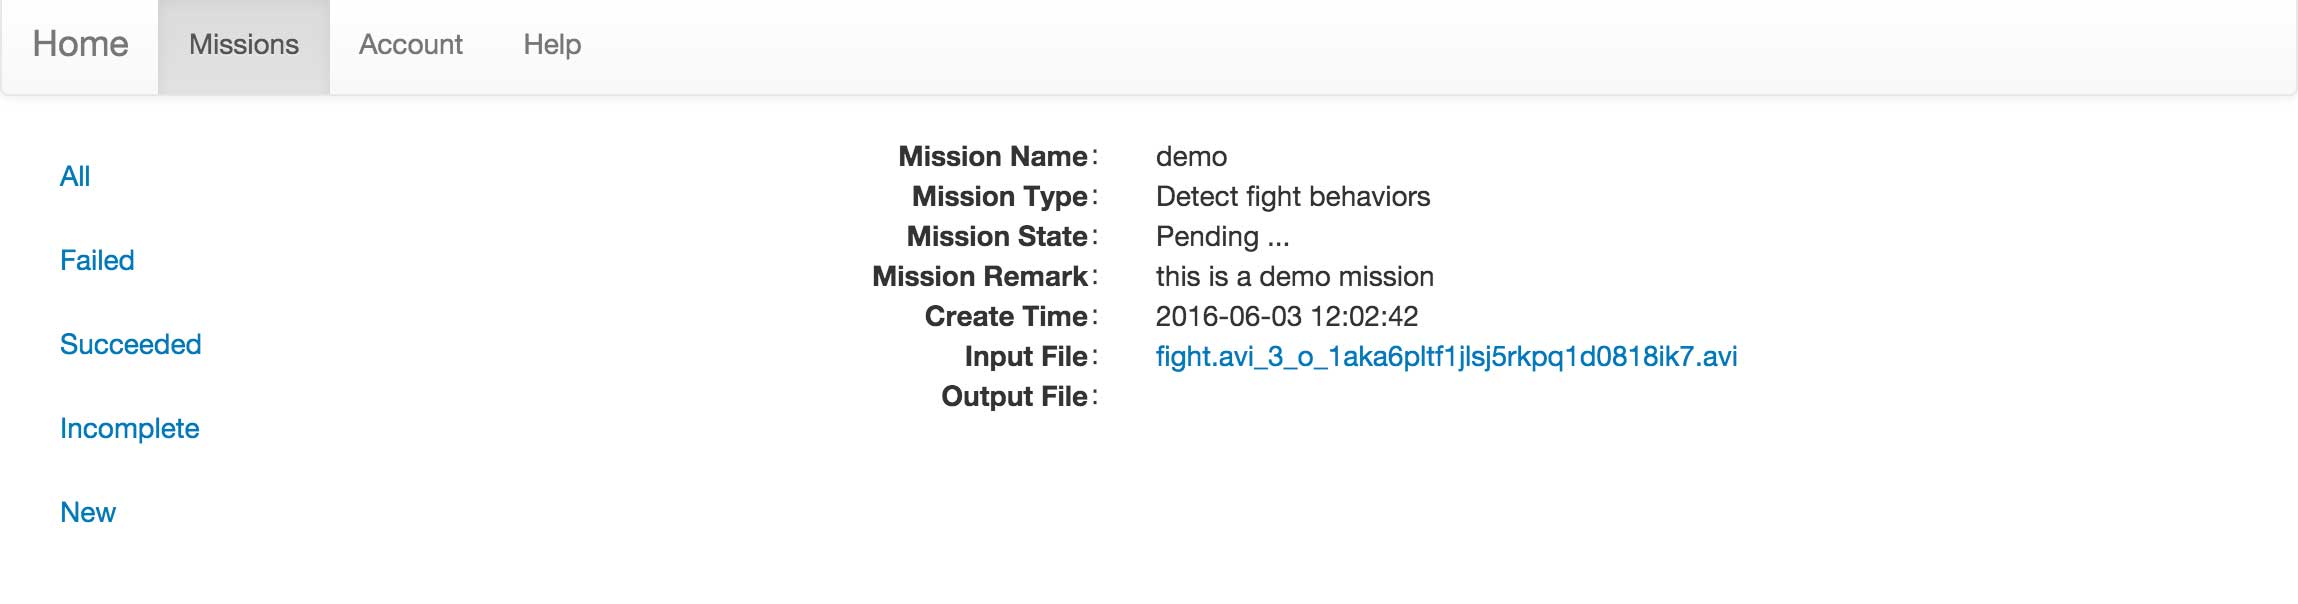
\includegraphics[width=0.8\textwidth]{website_waiting_for_result}
\caption{等待任务完成}
\label{fig:website_waiting_for_result}
\end{figure}

最后,经过任务队列的等待后,网站后台对任务进行分析,得到果蝇行为识别的结果,如图~\ref{fig:website_show_result}所示。

\begin{figure}
\centering
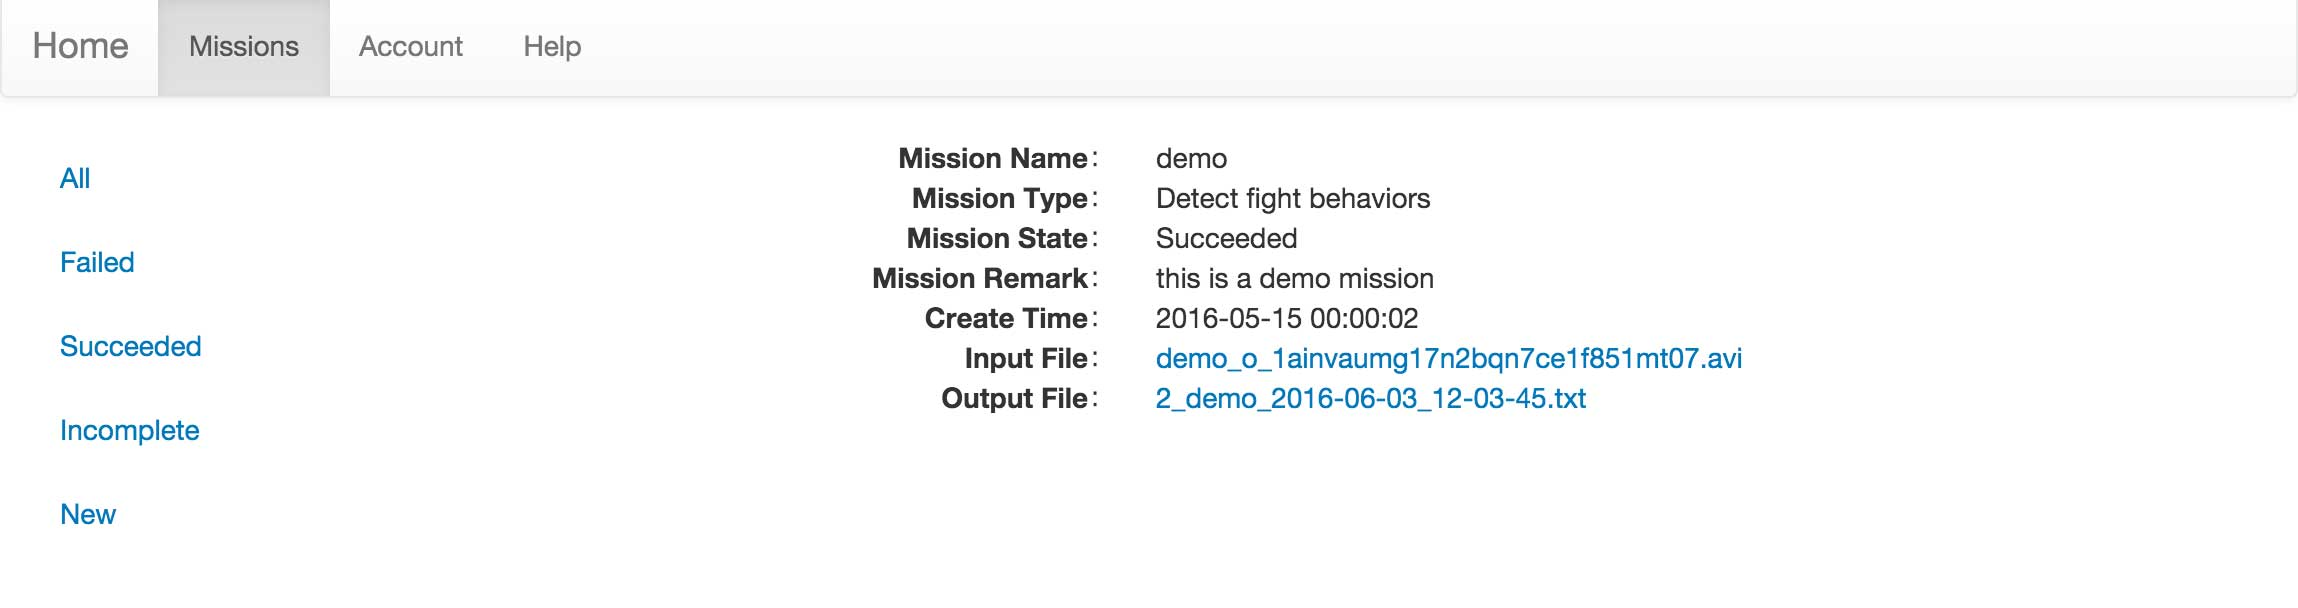
\includegraphics[width=0.8\textwidth]{website_show_result}
\caption{果蝇行为识别任务的结果}
\label{fig:website_show_result}
\end{figure}

图~\ref{fig:website_show_result}中,"Output File"栏目对应的就是果蝇行为识别的结果,即果蝇打架日志。对于不同类型的果蝇行为分析任务,其日志输出有不同的格式。对于打架行为,日志的第一行统计了视频中果蝇的打架次数,其后有以下3列:
\begin{itemize}
\item time – 打架发生的时间
\item frame – 打架发生的帧数,和time对应(从零开始)
\item strength – 打架强度
\end{itemize}
对于果蝇的求偶行为,求偶行为包括果蝇的身体求偶行为和振翅求偶行为,日志的第一行统计了视频中的求偶行为总数,其后有以下4列:
\begin{itemize}
\item time – 求偶起始时间
\item start – 求偶起始帧(含)
\item end – 求偶结束帧(含)
\item behavior – 求偶行为
\end{itemize}

除基本的日志外,果蝇求偶行为分析日志文件还输出简单的统计信息。在输出身体求偶或振翅求偶行为后,日志输出各求偶行为的持续时间,包括:
\begin{itemize}
\item count – 行为总发生次数
\item duration – 行为总持续时间
\end{itemize}
最后,日志输出行为间的转移矩阵,其第$i$行第$j$列表示从第$j$个行为向第$i$个行为转移的次数,单位为帧。用户通过下载果蝇行为日志文件,并按照既定格式进行分析,得到果蝇行为的各项参数,用于支持果蝇行为学的研究。

\subsection{果蝇行为识别网站简介}

网站建设在Ubuntu 14.04系统上,操作系统的选择主要考虑了果蝇行为识别程序的发布、网站服务的搭建等,最后综合选取了Ubuntu 14.04操作系统。网站的基本环境要求如下:
\begin{itemize}
    \item 操作系统:Ubunutu 14.04
    \item Web服务器: Apache2,支持PHP
    \item PHP: >=5.2.4
    \item 数据库:MySQL 5.5
    \item Python: 2.7.x
\end{itemize}

网站部分使用CodeIgniter框架搭建。CodeIgniter是一个轻量级的MVC架构的php网站框架,基于MVC模型,将网站的应用层和逻辑层进行分离\cite{burbeck87}。关于后台的数据库,系统使用MySQL数据库存储数据,主要存储了包括用户账户相关的数据表、任务类型数据表、任务数据表等,分别参见表~\ref{tab:account}、表~\ref{tab:mission_type}和表~\ref{tab:misson}。

\begin{table}
\centering
\caption{账户信息数据表dp\_account}
\label{tab:account}
\begin{tabular}{ccc}
\toprule[1.5pt]
字段名 & 字段类型 & 备注 \\ \midrule[1pt]
aid & bigint(20) & Unsigned, Primary key, Auto Increment \\
state & tinyint(4) & 0:等待审核,1:正常,2:禁用 \\
username & varchar(20) & 用户名 \\
password & varchar(32) & 密码的md5 \\
work\_unit & varchar(255) & 学校/单位 \\
department & varchar(255) & 院系 \\
purpose & varchar(255) & 实验目的 \\
source & varchar(255) & 项目来源 \\
data\_amount & varchar(255) & 数据量 \\
create\_time & timestamp & 默认current\_timestamp \\ \bottomrule[1.5pt]
\end{tabular}
\end{table}

\begin{table}
\centering
\caption{任务类型数据表dp\_missiontype}
\label{tab:mission_type}
\begin{tabular}{ccc}
\toprule[1.5pt]
字段名 & 字段类型 & 备注 \\ \midrule[1pt]
mtid & int(10) & Unsigned, Primary key, Auto Increment \\
state & tinyint(3) & 0:Invalid, 1:Valid \\
typename & varchar(255) & 类型名称 \\
description & varchar(1000) & 类型说明 \\
command & varchar(255) & 处理命令,可以加入特殊符号,具体见下表 \\
in\_file\_exts & varchar(255) & 允许的输入文件后缀,逗号分隔 \\
out\_file\_ext & varchar(10) & 输出文件的后缀 \\
max\_in\_file\_size & varchar(20) & 允许上传的输入文件大小 \\
error\_messages & varcahr(1000) & json格式字符串,各个error\_code的含义 \\ \bottomrule[1.5pt]
\end{tabular}
\end{table}

\begin{table}
\centering
\caption{任务数据表dp\_mission}
\label{tab:misson}
\begin{tabular}{ccp{0.5\columnwidth}}
\toprule[1.5pt]
字段名 & 字段类型 & 备注 \\ \midrule[1pt]
mid & bigint(20) & Unsigned, Primary key, Auto Increment \\
aid & bigint(20) & 所属account的aid \\
type & mediumint(6) & 任务类型的id,对应dp\_missiontype中的mtid \\
name & varchar(20) & 任务名称 \\
remark & varchar(1000) & 任务备注 \\
state & smallint(6) & {任务状态,
\begin{itemize}
    \item 0 : Pending等待处理
    \item 1 : Proceeding处理中
    \item 2 : Succeeded
    \item 3 : Failed
\end{itemize}} \\
error\_code & int(11) & 错误码,状态为Failed时有效 \\
in\_file\_path & varchar(255) & 输入文件路径,相对于项目根目录 \\
out\_file\_path & varchar(255) & 输出文件路径,相对于项目根目录,状态为Succeeded时有效 \\
stdout\_file\_path & varchar(255) & 处理过程的stdout日志文件路径,相对于项目根目录,状态为Succeeded/Failed时有效 \\
stderr\_file\_path & varchar(255) & 处理过程的stderr日志文件路径,相对于项目根目录,状态为Succeeded/Failed时有效 \\
create\_time & timestamp & 创建时间,默认current\_timestamp \\
complete\_time & datetime & 完成时间,状态为Succeeded/Failed时有效 \\
\bottomrule[1.5pt]
\end{tabular}
\end{table}

任务处理使用Python脚本实现,并用Supervisor管理脚本的执行。Supervisor是一个基于Python的进程管理系统,可以方便的进行任务的创建、监听、重启、崩溃恢复等,经过简单的配置后,可以用Supervisor进行任务队列的管理,安排果蝇自动检测程序DetectFly对果蝇视频的任务队列进行逐个分析和处理。通过为不同的任务类型指定不同的命令行参数,调用DetectFly程序,完成果蝇行为的识别,并将行为识别的结果保存为日志文件,方便用户下载和分析。

\section{小结}

在Ubuntu下配置开发环境,得到果蝇行为自动识别的可执行程序DetectFly。DetectFly可以通过命令行参数,实现不同类型的果蝇行为识别。在CodeIgniter框架的基础上,使用Supervisor进行任务队列管理,最终实现了果蝇行为识别网站的任务管理。


% \chapter{总结与展望}

\section{论文工作总结}

动物行为学是生物学研究中的重要领域,而果蝇行为学是动物行为学中的一个分支。果蝇因其形态简单等原因,可以通过计算机视觉、机器学习等相关领域的技术对果蝇进行自动识别。本文为了提高果蝇行为识别对视频拍摄环境变化的鲁棒性,针对果蝇行为识别的果蝇活动台分割和果蝇身体轮廓提取部分进行研究,并以网站的形式提供果蝇行为检测服务。下面是本文的主要工作和创新点。

首先,果蝇活动台的分割操作一般通过对形态学上检测来完成,匹配的检测果蝇活动台的形状来提取果蝇活动台的位置。为了适应不同果蝇行为视频的差异,本文通过对形态学操作中的参数控制形检测到的形状的数目,并对参数进行自适应,提高了果蝇活动台匹配算法的适用性。同时,针对特定排列的果蝇活动台,通过对活动台的实际坐标和理想坐标之间建立仿射变换,提高了果蝇活动台位置的准确性。

其次,针对果蝇身体轮廓提取算法,本文在背景模型的基础上,通过对果蝇视频背景进行首次建模,得到初步的果蝇身体和翅膀提取算法,进而通过分离果蝇身体和翅膀,实现对果蝇活动台的单独建模,得到精确的果蝇活动台模型。上述背景模型显著提高了果蝇身体轮廓提取的鲁棒性,在不同的果蝇行为视频中表现出相当的鲁棒性。

最后,通过搭建网站,提供果蝇行为识别的服务,可以方便不同研究人员使用相关的服务。

\section{未来工作展望}

基于本文开展的工作,将来的工作可以有以下几个考量:

\begin{enumerate}
\item 目前,本文仅针对果蝇活动台分割和果蝇身体轮廓提取部分进行了充分的实验,对于背景模型和果蝇行为识别的准确率之间的关系,受限于标定的果蝇视频的规模,目前还没有完全展开,希望以后能进一步在其他果蝇行为视频的数据上加以推广、验证。
\item 果蝇活动台分割算法的准确性还有待提高。对于排列不规则的果蝇活动台,对果蝇活动台中心进行聚类时偶尔会出现部分活动台被重复定位、部分活动台没有被准确定位到的问题,算法运行的结果还需要手工进行确认。
\item 果蝇行为分析的效率还存在提升的空间,目前在算法层面上可以改进的空间相对不多,可以用GPU运算等方式提高检测程序的处理能力。
\item 可以将对果蝇的背景模型等研究加以推广,应用到其他类型的研究中。
\end{enumerate}


%%% 其它部分
\backmatter

%% 本科生要这几个索引,研究生不要。选择性留下。
% 插图索引
% \listoffigures
% 表格索引
% \listoftables
% 公式索引
% \listofequations


%% 参考文献
% 注意:至少需要引用一篇参考文献,否则下面两行可能引起编译错误。
% 如果不需要参考文献,请将下面两行删除或注释掉。
\bibliographystyle{thuthesis}
\bibliography{ref/refs}

%% 致谢
\begin{acknowledgement}

我要感谢我的导师谷源涛老师,在我的研究生学习期间,谷老师在我的学术研究上给予了充分的指导,帮助我在自己的研究上有充分的发挥。同时,谷老师对我的职业规划和发展方向也给予了很多的建议和帮助,让我受益匪浅。此外,谷老师严谨求实的工作作风,勤奋认真的工作态度都潜移默化地感染了我。谷老师对于我的论文工作也提供了诸多指点和帮助,在此我要向谷老师表示由衷的感谢。

我要感谢实验室的各位同学,他们抽出宝贵的时间,帮助我对论文中的实验语音进行了主观质量标注。尤其要感谢刘雄飞同学,他参与了很多短波语音的采集工作,非常枯燥耗时,但对于本文工作又是至关重要的。

我还要感谢我的父母、家人和朋友。他们对我的关心和支持给了我不断突破自我的动力,特别要感谢段泽群同学一直以来的陪伴与关心。

\end{acknowledgement}


%% 附录
% \begin{appendix}
% \input{data/appendix01}
% \end{appendix}

%% 个人简历
\begin{resume}

\resumeitem{个人简历}

1994年2月4日生于江苏省淮安市。

2011年9月通过竞赛保送进入 清华大学 电子工程系 电子信息科学与技术专业,2015年7月本科毕业,并获得了工学学士学位,同时获得免试攻读 清华大学 电子工程系 工学硕士学位资格。

2015年9月面试进入 清华大学 电子工程系 攻读 信息与通信工程专业 工学硕士学位 至今。

\researchitem{学术论文发表情况}

\begin{publications}
\item Ye Chen, Yongcheng Wang, Jiaguo Yang, Yuantao Gu. Automatic Switching Technique for Speech Enhancement in HF Communications. IEEE 8th International Conference on Electronics Information and Emergency Communication (已录用,EI)
\item 谷源涛,陈晔. 语音质量评价方法及装置. (已申请,专利)
\end{publications}

\end{resume}

\end{document}
